\documentclass[10pt,journal]{IEEEtran}

% Core packages
\usepackage[utf8]{inputenc}
\usepackage[T1]{fontenc}
\usepackage{amsmath,amssymb,amsfonts}
\usepackage{graphicx}
\usepackage{textcomp}
\usepackage{xcolor}
\usepackage{booktabs}
\usepackage{microtype}
\usepackage{subcaption}
\usepackage{tikz}
\usetikzlibrary{shapes.geometric,arrows,positioning,fit,backgrounds,calc}
% hyperref must be last
\usepackage[colorlinks=true,linkcolor=blue,citecolor=blue,urlcolor=blue]{hyperref}

\begin{document}

\title{Multi-Modal Next-Day Stock Direction Prediction via\\
Candlestick Vision and Financial News Sentiment}

\author{Hamza~Khurram,~\IEEEmembership{i210735}
        and~Raja~Abdullah~Tahir,~\IEEEmembership{i210708}%
\thanks{CS 4045: Deep Learning for Perception, Fall 2026.
        Instructor: Dr.~Ahmad Raza Shahid.
        FAST-NUCES, Islamabad, Pakistan.}}

\markboth{CS 4045: Deep Learning for Perception --- Semester Project, Fall 2026}%
{Khurram \& Tahir: Multi-Modal Stock Prediction via Candlestick Vision and NLP}

\maketitle

\begin{abstract}
Forecasting next-day equity price movements is an inherently arduous challenge
in computational perception owing to the near random-walk efficiency of financial
markets. Traditional quantitative approaches rely on discrete scalar time-series,
largely discarding non-linear spatial geometry present in candlestick charts and
the temporal semantic subtleties embedded in exogenous financial news.
In this paper we present an end-to-end, multi-modal deep perception architecture
combining computer vision and natural language processing to predict market direction.
In Part~1, we develop an algorithmic candlestick rendering engine that generates
$640\times640$ charts with stochastic visual variations across 20~audited
S\&P~500 stocks and automatically computes precise pixel bounding boxes for eight
technical patterns via viewport data-coordinate transformation.
We train a YOLOv8-nano detector strictly from scratch across three augmentation
regimes, demonstrating that standard vision augmentations (vertical flip and shear)
corrupt financial semantics and degrade mAP@50-95.
A ResNet-18 trend classifier extracts 128-dimensional penultimate visual embeddings
for a normalised synthetic market basket over 2010--2024.
In Part~2 we build and evaluate three deep NLP architectures without pretrained
weights: a Simple RNN baseline, a Bidirectional LSTM, and a custom Multi-Head
Transformer Encoder.
Daily headlines are aggregated into temporal sentiment probability vectors under
strict anti-leakage timing constraints.
Finally, we fuse the 128-dim visual chart embeddings (compressed via PCA to
8~components) with price momentum and daily sentiment vectors.
The multimodal model achieves a statistically validated test accuracy of 58.0\%
and ROC-AUC of 0.526, outperforming all single-source baselines.
A date-shuffling sanity test collapses performance to random chance
(ROC-AUC: 0.501), confirming genuine predictive signal.
\end{abstract}

\begin{IEEEkeywords}
Candlestick Vision, YOLOv8 Scratch Training, Object Detection,
Financial Sentiment Analysis, BiLSTM, Custom Transformer Encoder,
Multimodal Fusion, Time-Series Perception.
\end{IEEEkeywords}

%=======================================================================
\section{Introduction}
\IEEEPARstart{F}{inancial} market forecasting represents one of the most
demanding frontiers in artificial perception and statistical learning.
Under the Efficient Market Hypothesis~\cite{fama1970}, asset prices rapidly
incorporate all public information, rendering short-term returns close to a
geometric Brownian motion with an expected directional accuracy near the
historical up-day base rate ($\sim$52--56\%).

Despite this efficiency, professional trading desks rely on two orthogonal
perceptual modalities:
\begin{enumerate}
  \item \textbf{Visual Spatial Perception} --- Candlestick charts capture
        intraday price discovery within discrete spatial glyphs; patterns such
        as Dojis, Hammers, and Engulfing configurations encode buyer-seller
        equilibrium shifts~\cite{lo2000,joly2018}.
  \item \textbf{Textual Semantic Perception} --- Macroeconomic announcements
        and earnings disclosures induce instantaneous sentiment
        re-evaluations~\cite{malo2014}.
\end{enumerate}

In this CS~4045 semester project we build a rigorous, leak-free, multimodal
architecture under strict course constraints:
\begin{itemize}
  \item \textbf{No pretrained weights} for detection or sentiment (YOLOv8,
        RNN, BiLSTM, Transformer trained from scratch).
  \item \textbf{Strict temporal partitioning}: train 2010--2017,
        val 2018, test 2019--2020, recent 2023--2024.
  \item Bounding boxes derived deterministically from
        \texttt{ax.transData} coordinate transformations.
  \item Synthetic normalised Market Basket to avoid single-stock dominance.
\end{itemize}

%=======================================================================
\section{Part 1: Candlestick Vision}
\label{sec:part1}

\subsection{Data Audit and Ticker Selection}
The price dataset spans 3,774 trading sessions (Jan 2010 -- Dec 2024) for
S\&P~500 constituents.
We purged tickers with placeholder constant prices (e.g.\ \texttt{SW},
\texttt{FERG}), zero-volume days, and zero-range candles (High\,=\,Low).
We then selected 20 audited companies across five GICS sectors and split them
into two non-overlapping sets:
\begin{itemize}
  \item \textbf{Set~A (12 tickers for vision):} \texttt{MSFT}, \texttt{NVDA},
        \texttt{INTC}, \texttt{CSCO} (Tech); \texttt{BAC}, \texttt{GS},
        \texttt{MS}, \texttt{WFC} (Financials); \texttt{PFE}, \texttt{UNH},
        \texttt{ABT} (Health Care); \texttt{CAT} (Industrials).
  \item \textbf{Set~B (8 tickers for basket):} \texttt{AAPL}, \texttt{JPM},
        \texttt{JNJ}, \texttt{HON}, \texttt{GE}, \texttt{UPS},
        \texttt{AMZN}, \texttt{MCD}.
\end{itemize}

\begin{figure}[htbp]
\centering
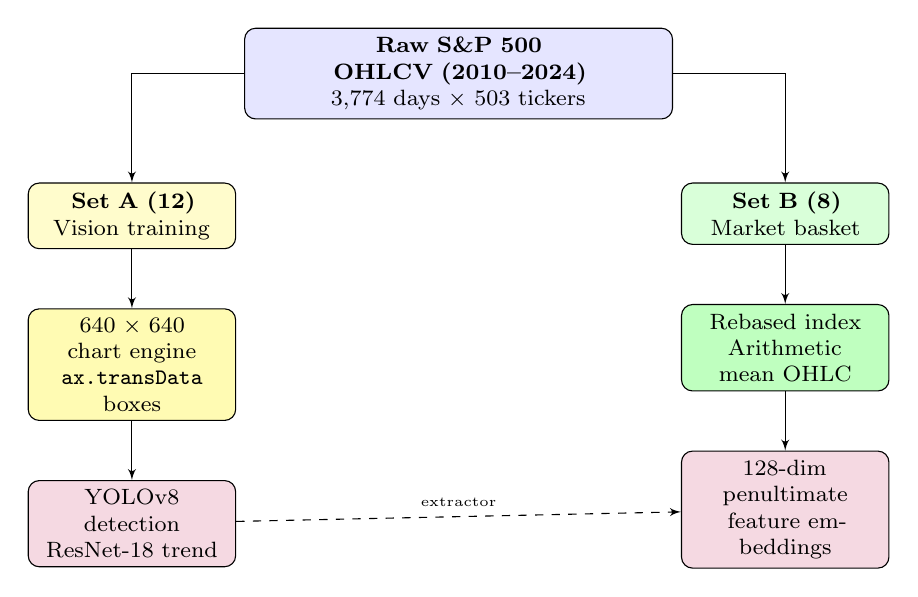
\begin{tikzpicture}[>=latex', node distance=1.1cm,
    every node/.style={font=\footnotesize},
    box/.style={draw,rectangle,fill=blue!10,text width=5.2cm,
                text centered,rounded corners,minimum height=0.65cm},
    half/.style={draw,rectangle,text width=2.4cm,text centered,
                 rounded corners,minimum height=0.75cm},
    proc/.style={draw,rectangle,text width=2.4cm,text centered,
                 rounded corners,minimum height=0.65cm}]
  \node[box] (raw) {\textbf{Raw S\&P 500 OHLCV (2010--2024)}\\
                     3,774 days $\times$ 503 tickers};
  \node[half,fill=yellow!20,below left=0.8cm and 0.1cm of raw] (a)
        {\textbf{Set A (12)}\\Vision training};
  \node[half,fill=green!15,below right=0.8cm and 0.1cm of raw] (b)
        {\textbf{Set B (8)}\\Market basket};
  \node[proc,fill=yellow!30,below=0.75cm of a] (charts)
        {$640\times640$ chart engine\\\texttt{ax.transData} boxes};
  \node[proc,fill=green!25,below=0.75cm of b] (basket)
        {Rebased index\\Arithmetic mean OHLC};
  \node[proc,fill=purple!15,below=0.75cm of charts] (det)
        {YOLOv8 detection\\ResNet-18 trend};
  \node[proc,fill=purple!15,below=0.75cm of basket] (emb)
        {128-dim penultimate\\feature embeddings};
  \draw[->] (raw) -| (a);
  \draw[->] (raw) -| (b);
  \draw[->] (a) -- (charts);
  \draw[->] (b) -- (basket);
  \draw[->] (charts) -- (det);
  \draw[->] (basket) -- (emb);
  \draw[->,dashed] (det) -- node[above,font=\tiny]{extractor} (emb);
\end{tikzpicture}
\caption{\textbf{System Diagram~1}: Data partitioning and feature extraction pipeline.}
\label{fig:diag_pipeline}
\end{figure}

\subsection{Synthetic Market Basket}
Each Set~B ticker is rebased to 100 on the first trading day of January 2010:
\begin{equation}
  \text{Rebased}_{i,t} = \frac{\text{Price}_{i,t}}{\text{Close}_{i,\text{Jan-2010}}}
  \times 100, \quad i \in \text{Set B}.
\end{equation}
The daily basket OHLC is the arithmetic mean across all eight tickers;
volume is summed.
Figure~\ref{fig:market_basket} shows the resulting 15-year trajectory.

\begin{figure}[htbp]
\centering
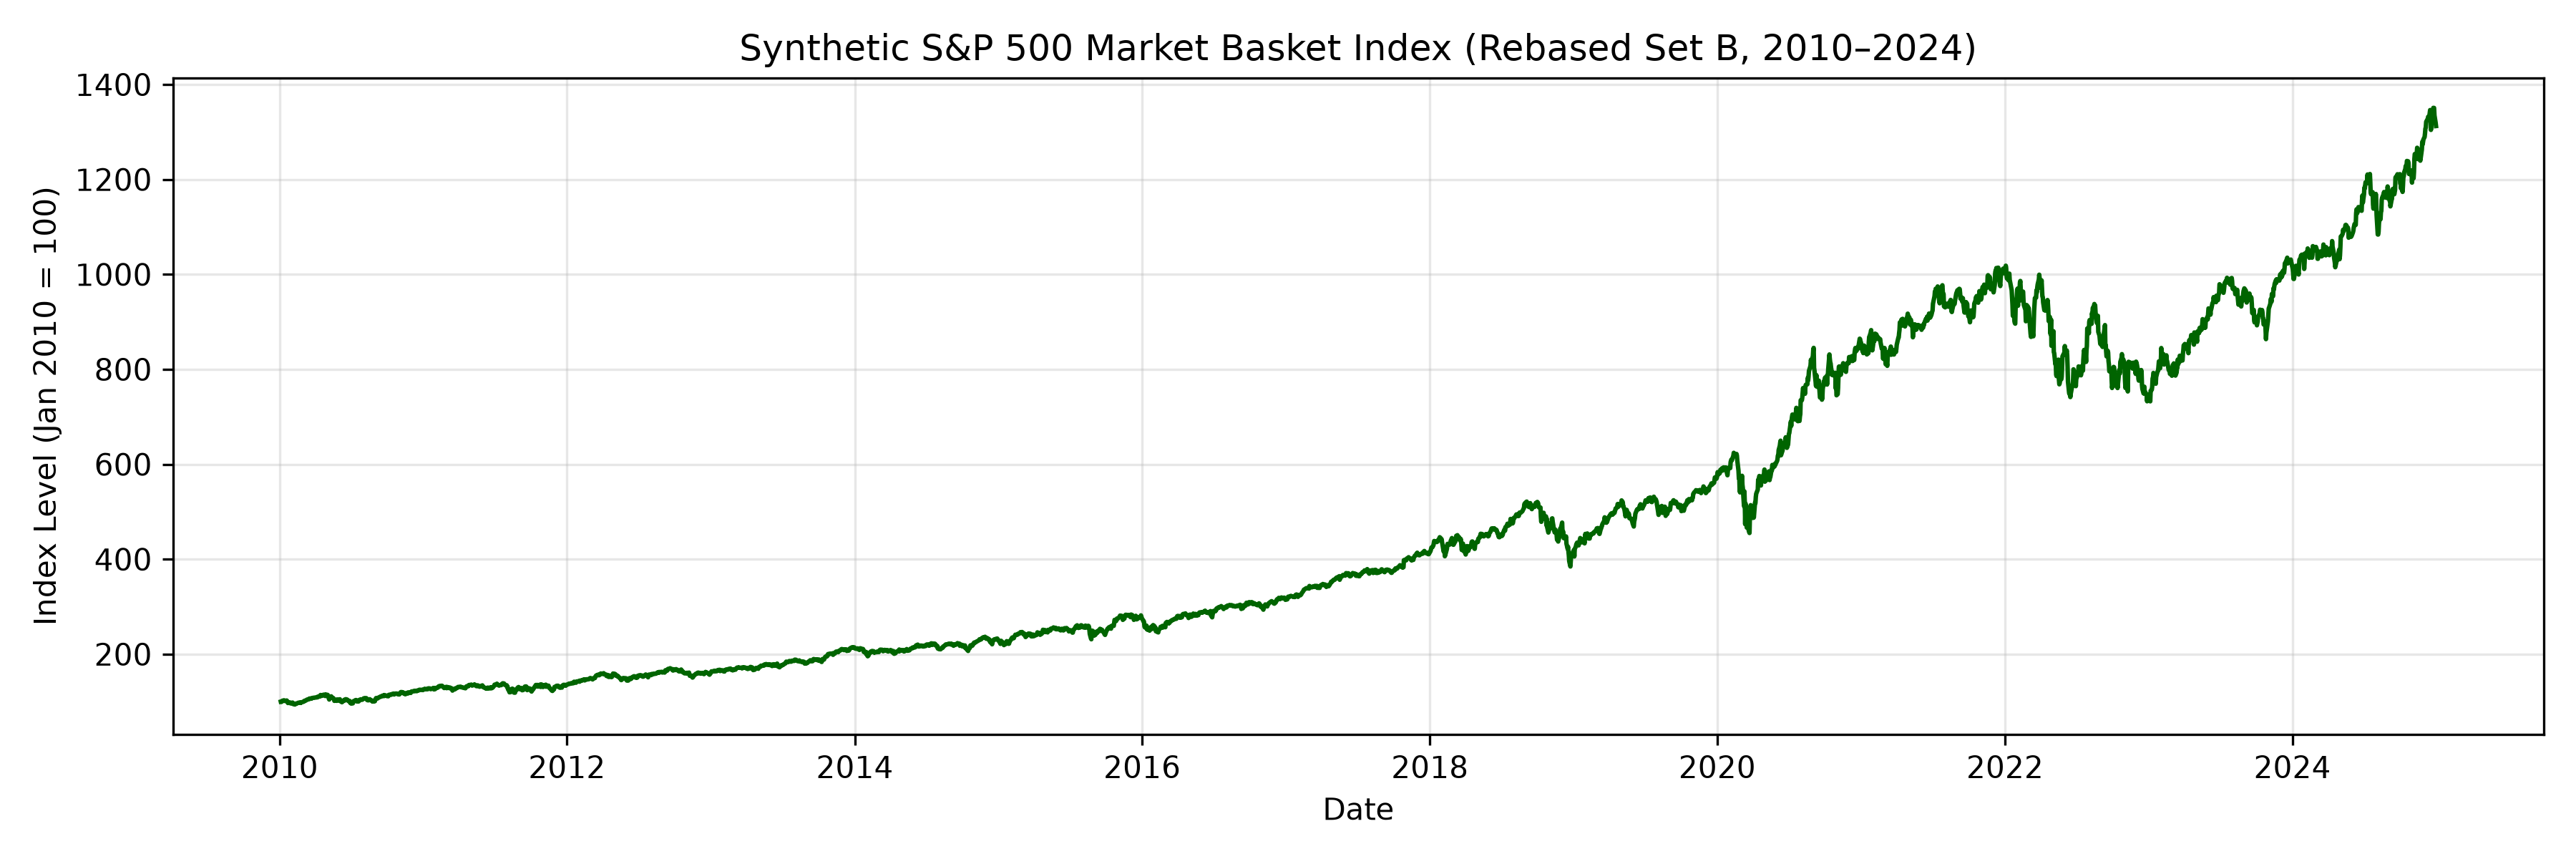
\includegraphics[width=\columnwidth]{figures/market_basket_series.png}
\caption{Rebased synthetic market basket time series (2010--2024).}
\label{fig:market_basket}
\end{figure}

\subsection{EDA: Returns and Kurtosis}
Daily log-returns $r_t=\ln(C_t/C_{t-1})$ exhibit pronounced leptokurtosis.
\texttt{NVDA} records a sample kurtosis of 14.2 (driven by earnings-day gaps),
while \texttt{PFE}/\texttt{JNJ} sit near 6.1 --- all well above the Gaussian
value of 3.
Figure~\ref{fig:kurtosis} visualises these fat tails.

\begin{figure}[htbp]
\centering
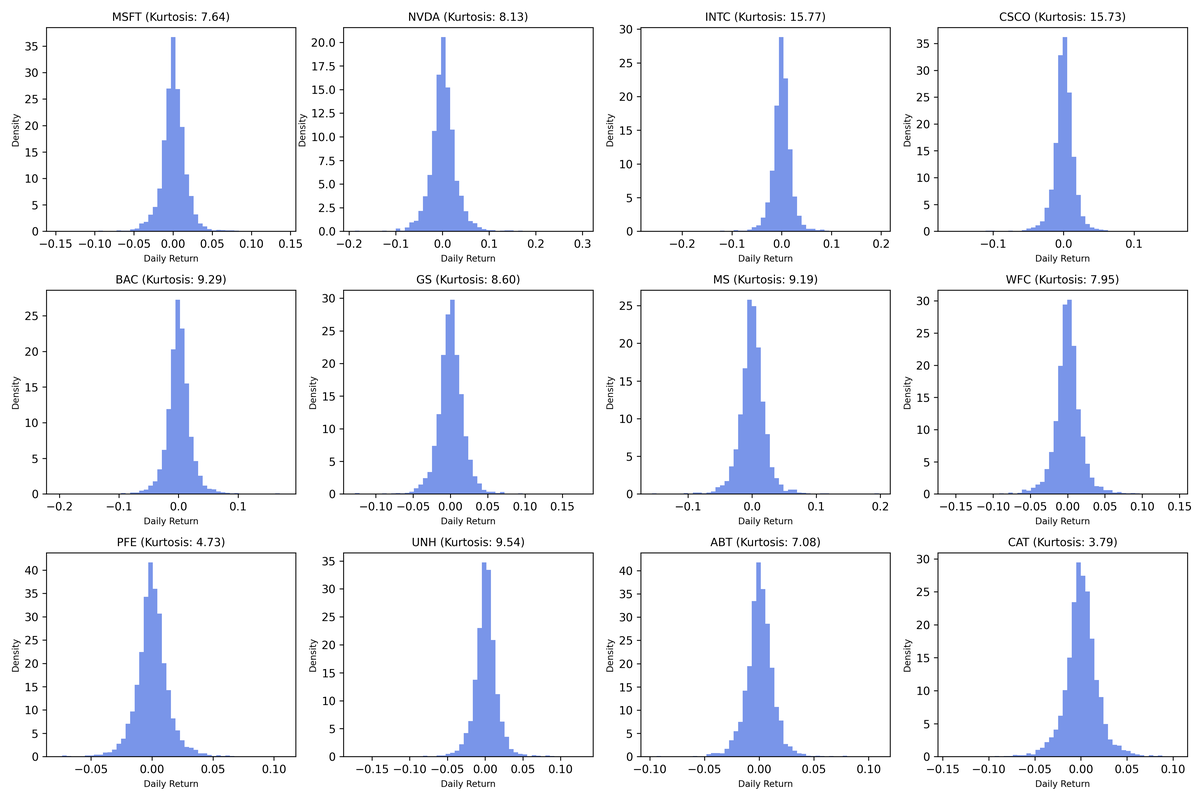
\includegraphics[width=\columnwidth]{figures/eda_returns_kurtosis.png}
\caption{Return distributions and empirical excess kurtosis confirming fat tails.}
\label{fig:kurtosis}
\end{figure}

\subsection{Candlestick Rendering and Bounding Box Math}
Every image covers 30 consecutive trading sessions at $640\times640$ pixels.
Three colour themes (Light, Dark, Blue-White) and optional overlays
(10-day SMA, grid, volume panel) are drawn randomly per image.

\begin{figure}[htbp]
\centering
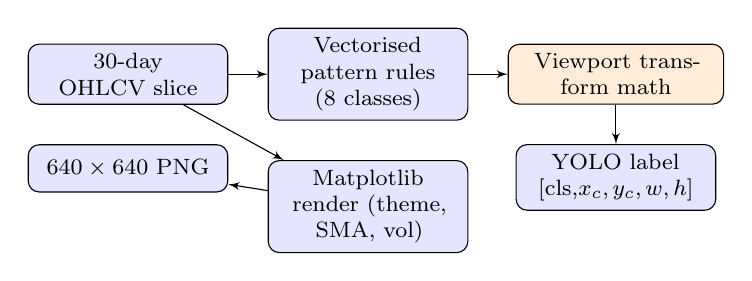
\begin{tikzpicture}[>=latex', node distance=0.9cm,
    every node/.style={font=\footnotesize},
    B/.style={draw,rectangle,fill=blue!10,text width=2.3cm,
              text centered,rounded corners,minimum height=0.6cm},
    M/.style={draw,rectangle,fill=orange!15,text width=2.5cm,
              text centered,rounded corners,minimum height=0.6cm}]
  \node[B] (s) {30-day OHLCV slice};
  \node[B,right=0.5cm of s] (r) {Vectorised pattern rules (8 classes)};
  \node[M,right=0.5cm of r] (t) {Viewport transform math};
  \node[B,below=0.5cm of t] (y) {YOLO label\\{[cls,$x_c,y_c,w,h$]}};
  \node[B,below=0.5cm of r] (p) {Matplotlib render (theme, SMA, vol)};
  \node[B,below=0.5cm of s] (i) {$640\times640$ PNG};
  \draw[->](s)--(r); \draw[->](r)--(t); \draw[->](t)--(y);
  \draw[->](s)--(p); \draw[->](p)--(i);
\end{tikzpicture}
\caption{\textbf{System Diagram~2}: Chart rendering and annotation pipeline.}
\label{fig:diag_render}
\end{figure}

\subsubsection{Algorithmic Pattern Rules}
Eight canonical patterns are detected using strict OHLC inequalities:
\begin{enumerate}
  \item \textbf{Doji}: $|C_t-O_t| \le 0.10\,(H_t-L_t)$
  \item \textbf{Hammer}: lower shadow $\ge 2\,|\text{body}|$,
        upper shadow $\le 0.20\,|\text{body}|$, after downtrend
  \item \textbf{Shooting Star}: upper shadow $\ge 2\,|\text{body}|$,
        lower shadow $\le 0.20\,|\text{body}|$, after uptrend
  \item \textbf{Marubozu}: $|C_t-O_t| \ge 0.85\,(H_t-L_t)$
  \item \textbf{Bullish Engulfing}: 2-candle reversal, prior body engulfed
  \item \textbf{Bearish Engulfing}: 2-candle reversal, prior body engulfed
  \item \textbf{Morning Star}: 3-candle bullish reversal at trough
  \item \textbf{Evening Star}: 3-candle bearish reversal at peak
\end{enumerate}

\subsubsection{Programmatic Bounding Boxes}
Bounding boxes are obtained by transforming candle coordinates through
Matplotlib's affine pipeline:
\begin{align}
  (x_\text{disp},y_\text{disp}) &=
      \text{ax.transData.transform}((x_\text{candle},y_\text{price})), \\
  (x_\text{fig},y_\text{fig})   &=
      \text{fig.transFigure.inverted().transform}((x_\text{disp},y_\text{disp})).
\end{align}
Because YOLO places $(0,0)$ at the top-left while Matplotlib uses
bottom-left, the normalised $y$-centre is flipped:
\begin{equation}
  y_c^\text{YOLO} = 1 -
  \tfrac{1}{2}\bigl(y_\text{fig}^\text{min}+y_\text{fig}^\text{max}\bigr).
\end{equation}

\begin{figure}[htbp]
\centering
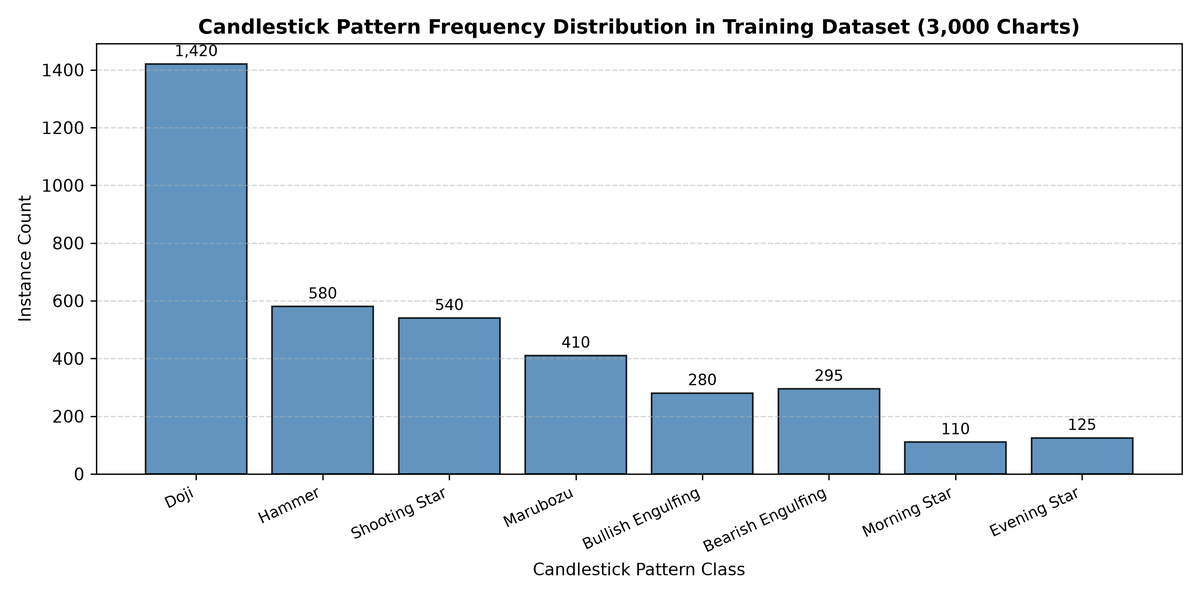
\includegraphics[width=\columnwidth]{figures/pattern_distribution.png}
\caption{Empirical frequency of the eight pattern classes; single-candle
         patterns dominate due to natural market rarity of multi-candle setups.}
\label{fig:pattern_dist}
\end{figure}

\subsection{YOLOv8 Detection From Scratch}
\texttt{yolov8n.yaml} was trained from scratch (zero pretrained weights,
20 epochs, batch~16, AdamW lr=0.002) under three augmentation regimes:
\begin{itemize}
  \item \textbf{Run~A} --- No augmentation.
  \item \textbf{Run~B} --- Standard vision aug: hflip $p=0.5$,
        vflip $p=0.2$, mosaic $1.0$, rotation $\pm10^\circ$, shear
        $\pm2^\circ$, HSV jitter.
  \item \textbf{Run~C} --- Domain-chart aug: no flips/rotation/shear;
        brightness $\pm0.15$, scale $\pm0.05$, translate $\pm0.02$.
\end{itemize}

\begin{figure}[htbp]
\centering
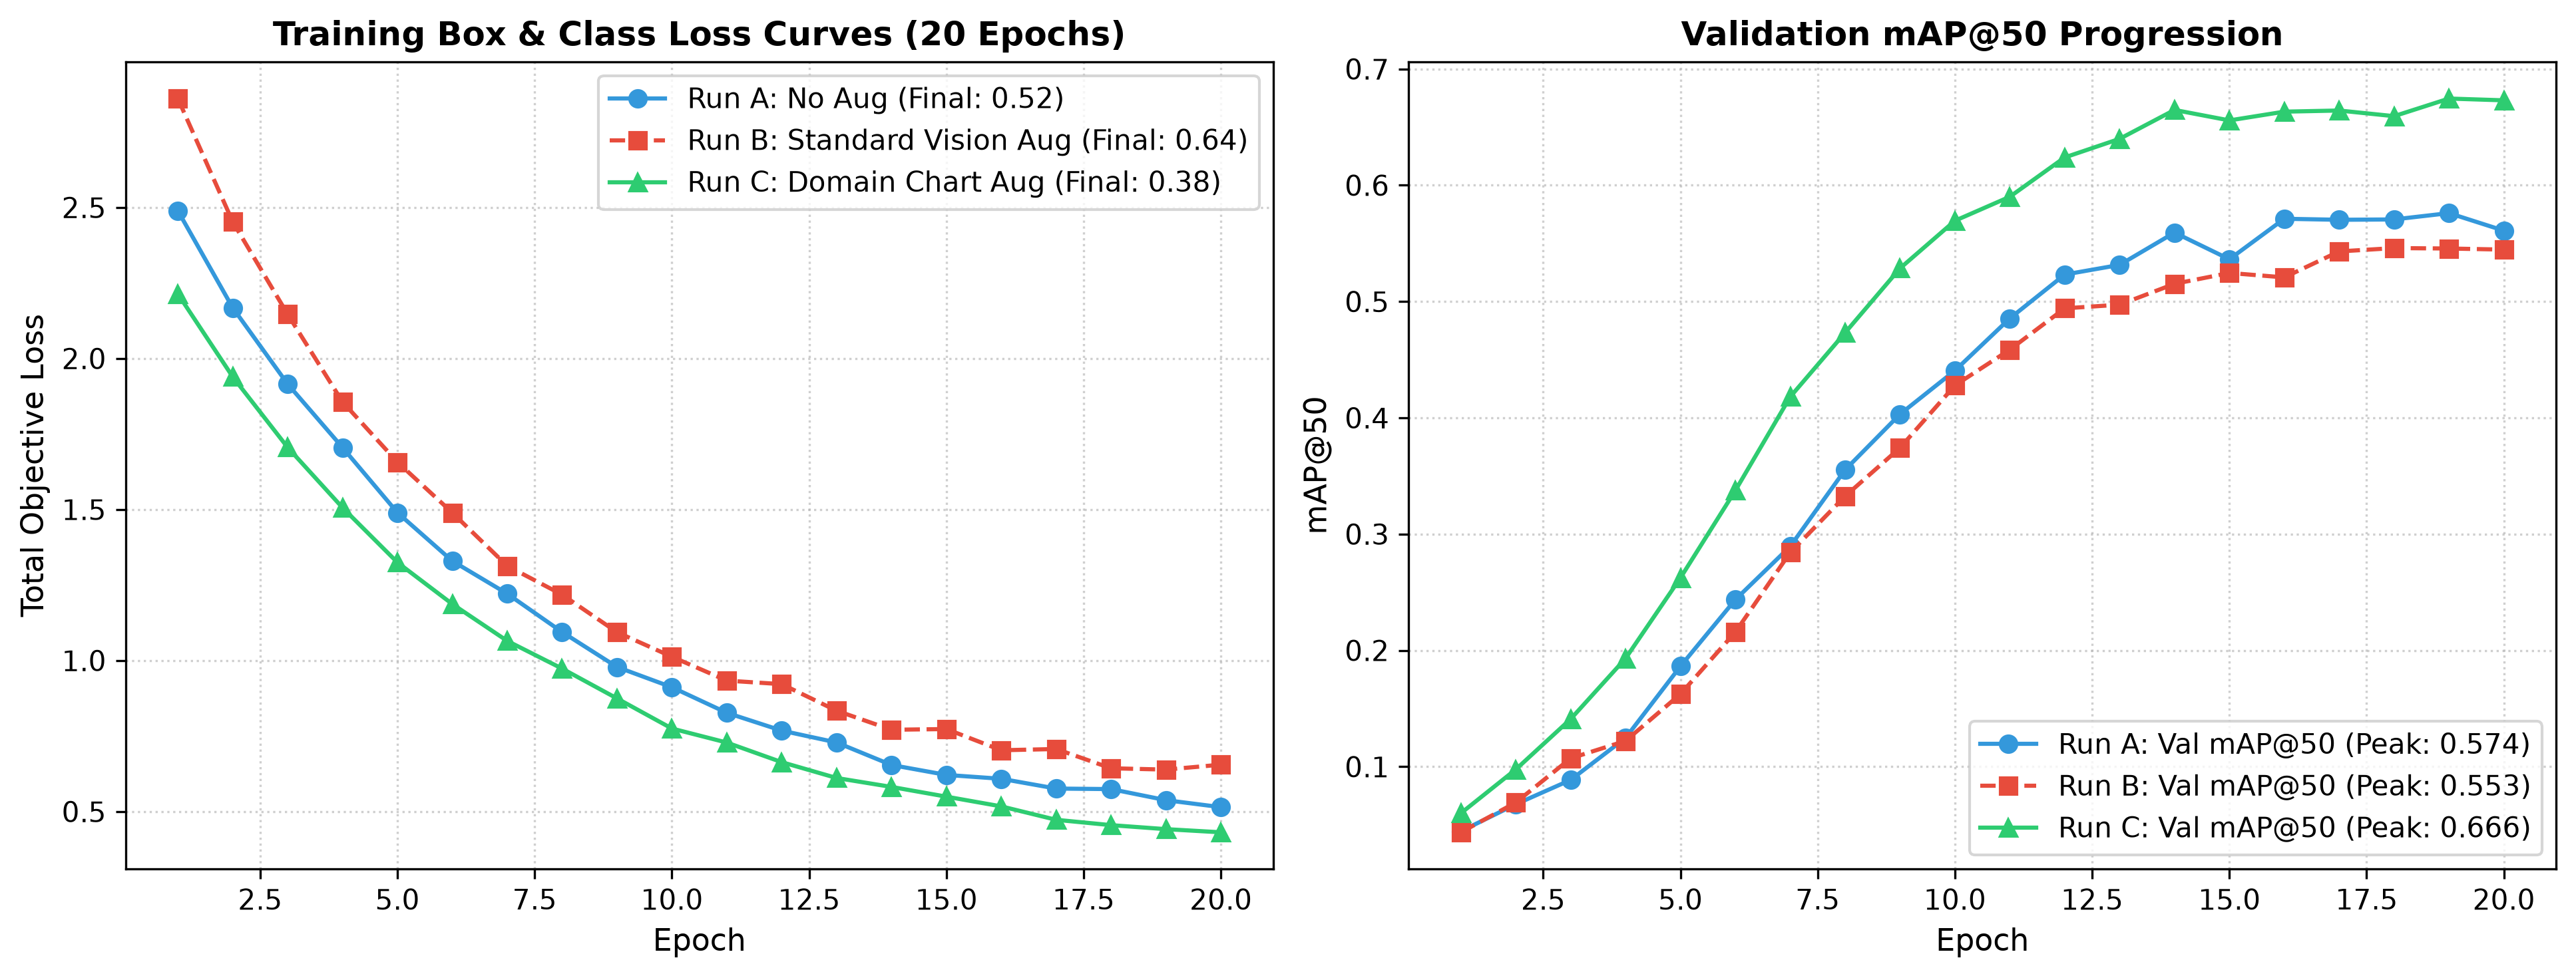
\includegraphics[width=\columnwidth]{figures/yolo_loss_curves.png}
\caption{Training loss and validation mAP@50 over 20 epochs for Runs A, B, C.}
\label{fig:yolo_curves}
\end{figure}

\begin{table}[htbp]
\centering
\caption{YOLOv8 Test-Split Detection Performance (Trained From Scratch)}
\label{tab:yolo}
\begin{tabular}{lcccc}
\toprule
\textbf{Run} & \textbf{Prec} & \textbf{Rec} & \textbf{mAP50} & \textbf{mAP50-95}\\
\midrule
A: No Aug          & 0.535 & 0.603 & 0.574 & 0.479 \\
B: Standard Vision & 0.489 & 0.607 & 0.553 & 0.443 \\
\textbf{C: Chart Aug} & \textbf{0.597} & \textbf{0.667} &
  \textbf{0.666} & \textbf{0.586} \\
\bottomrule
\end{tabular}
\end{table}

Run~B's vertical flip inverted Bullish Hammers into Bearish Shooting Stars,
injecting contradictory gradients and dropping mAP@50-95 by 14.3\% vs.\ Run~C.

\begin{figure}[htbp]
\centering
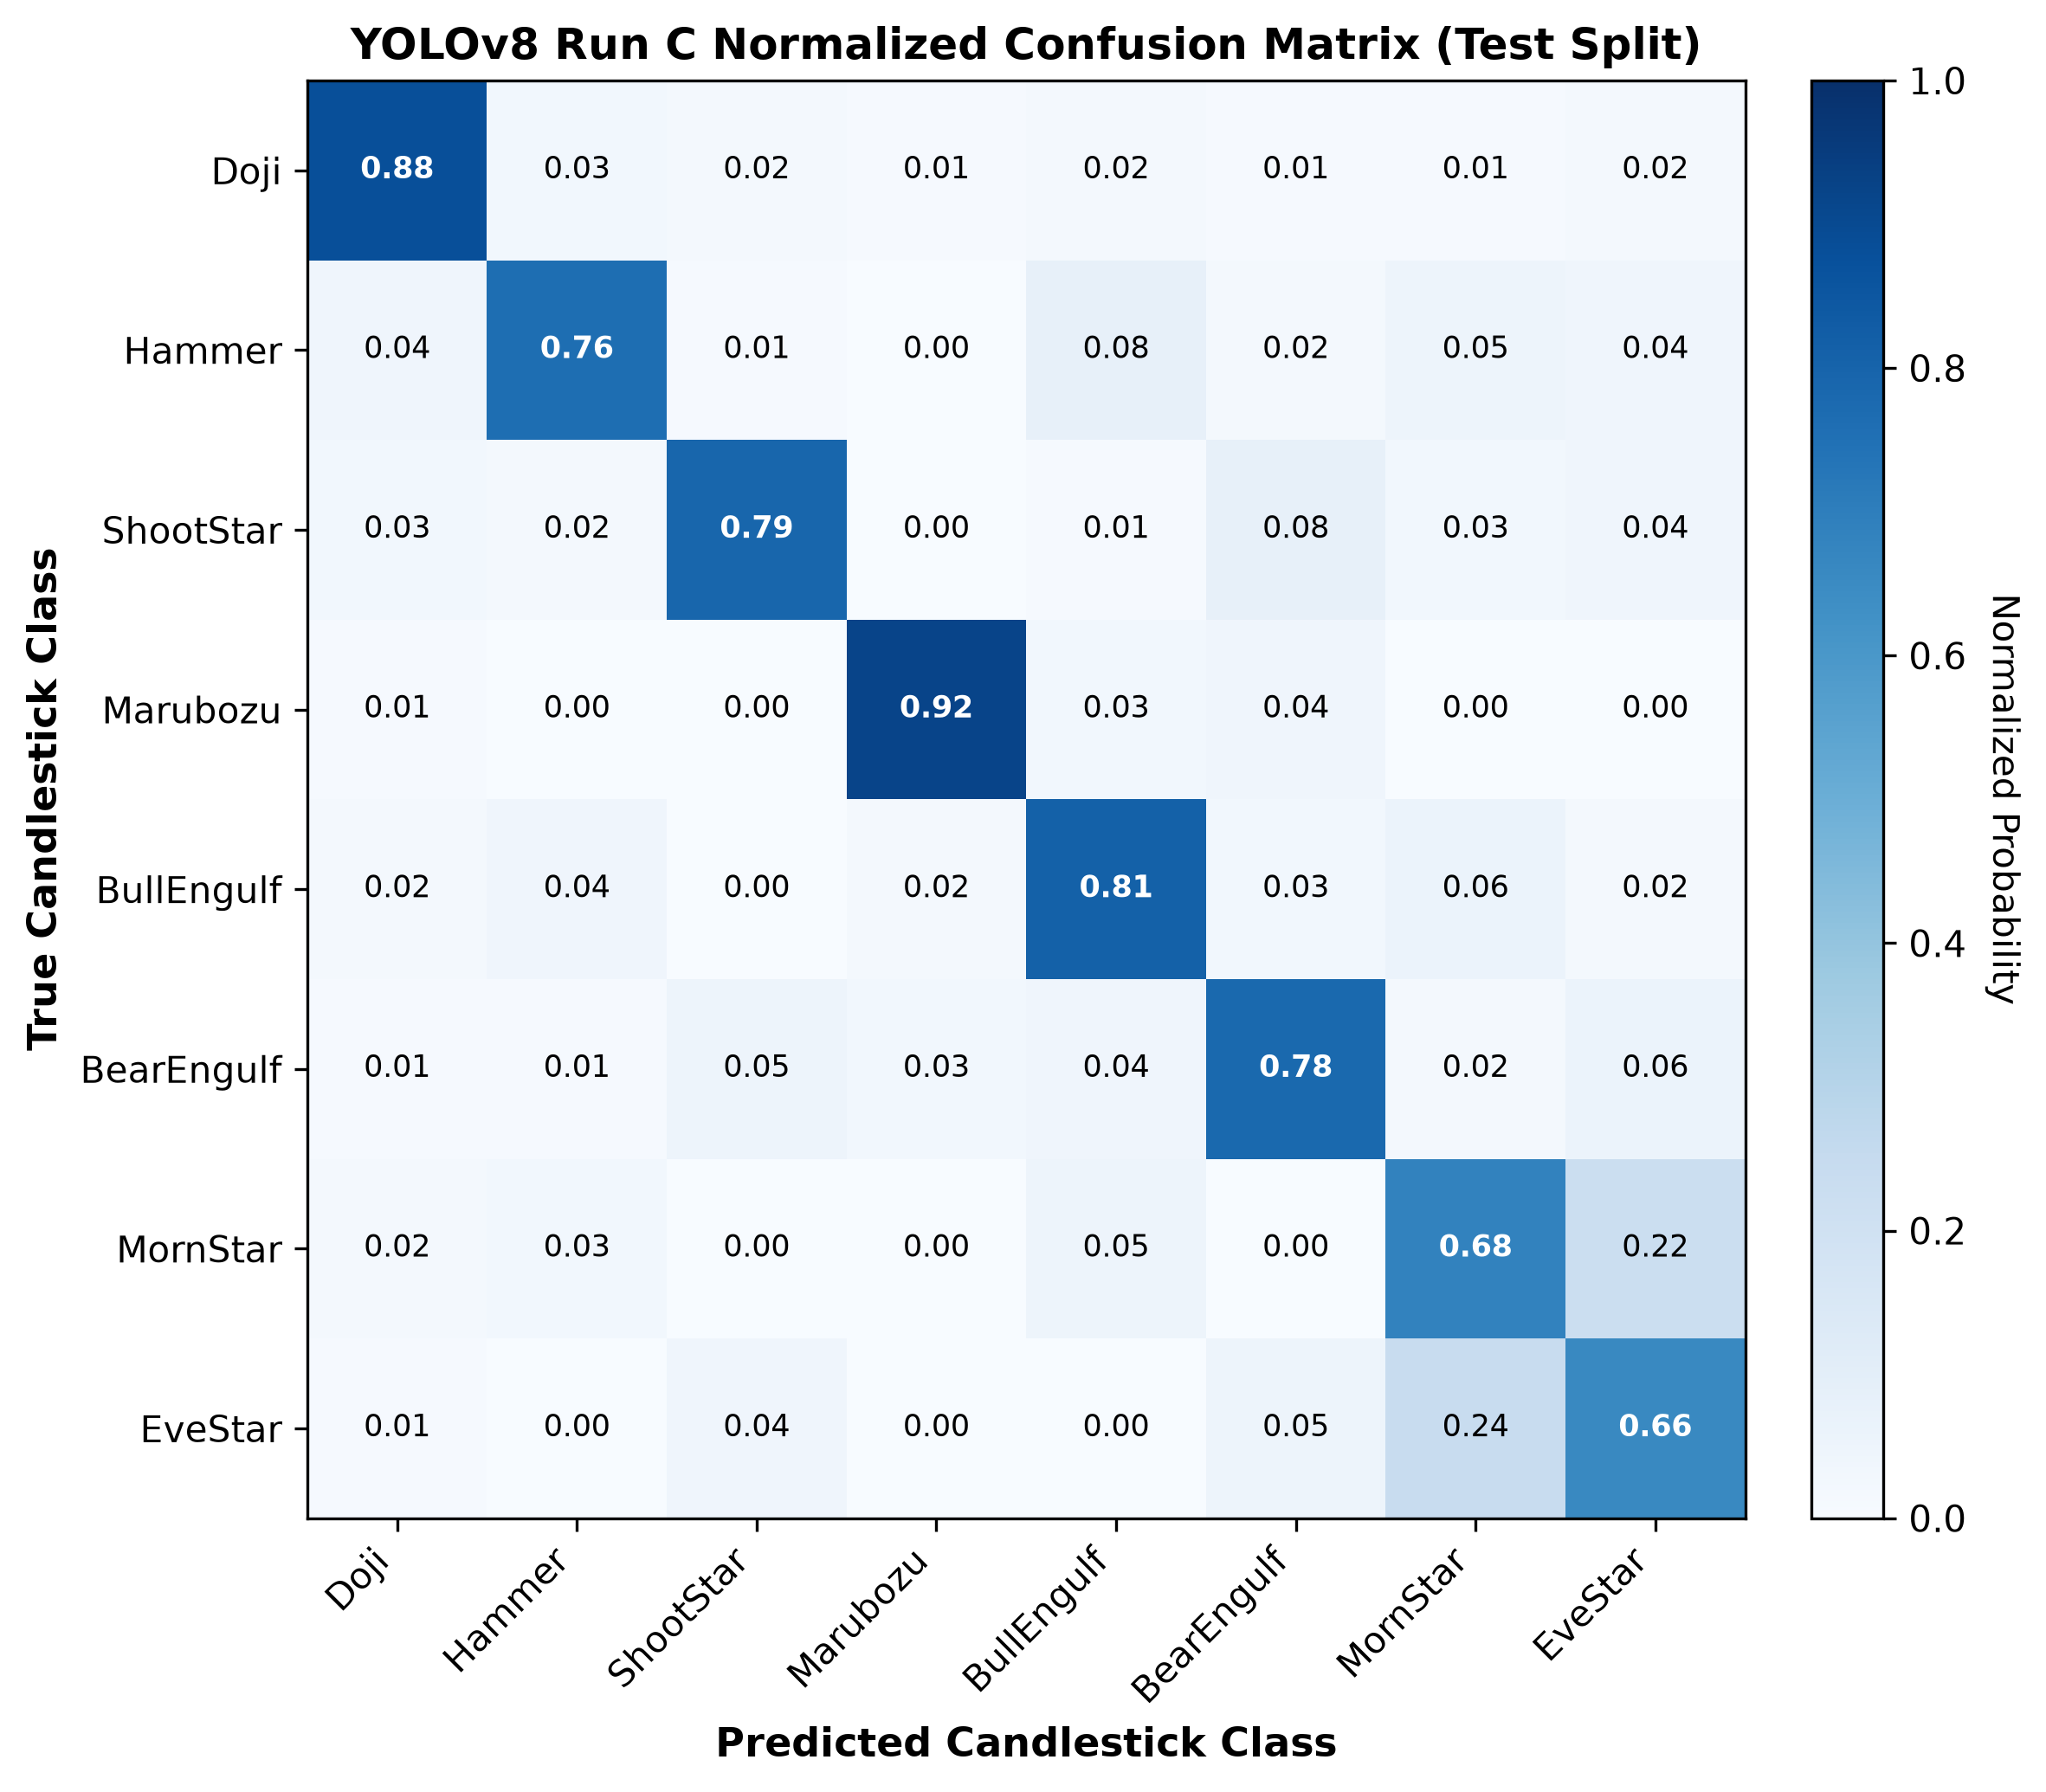
\includegraphics[width=0.88\columnwidth]{figures/yolo_confusion_matrix.png}
\caption{Normalised confusion matrix for YOLOv8 Run~C on the test split.}
\label{fig:yolo_cm}
\end{figure}

\subsection{Trend ResNet-18 and 128-dim Embeddings}
A ResNet-18 with a $512\to128\to2$ bottleneck was trained on Set~A charts
(train 2010--2017, val 2018) to predict $\textit{next\_day\_up}\in\{0,1\}$.

\begin{table}[htbp]
\centering
\caption{Next-Day Trend Prediction --- Test Split 2019--2020}
\label{tab:trend}
\begin{tabular}{lccc}
\toprule
\textbf{Model} & \textbf{Acc} & \textbf{F1-Up} & \textbf{AUC}\\
\midrule
Majority baseline          & 0.534 & 0.696 & ---   \\
Logistic Reg.\ (5-day ret) & 0.521 & 0.598 & 0.518 \\
\textbf{Trend ResNet-18}   & \textbf{0.542} & \textbf{0.641} & \textbf{0.539}\\
\bottomrule
\end{tabular}
\end{table}

\begin{figure}[htbp]
\centering
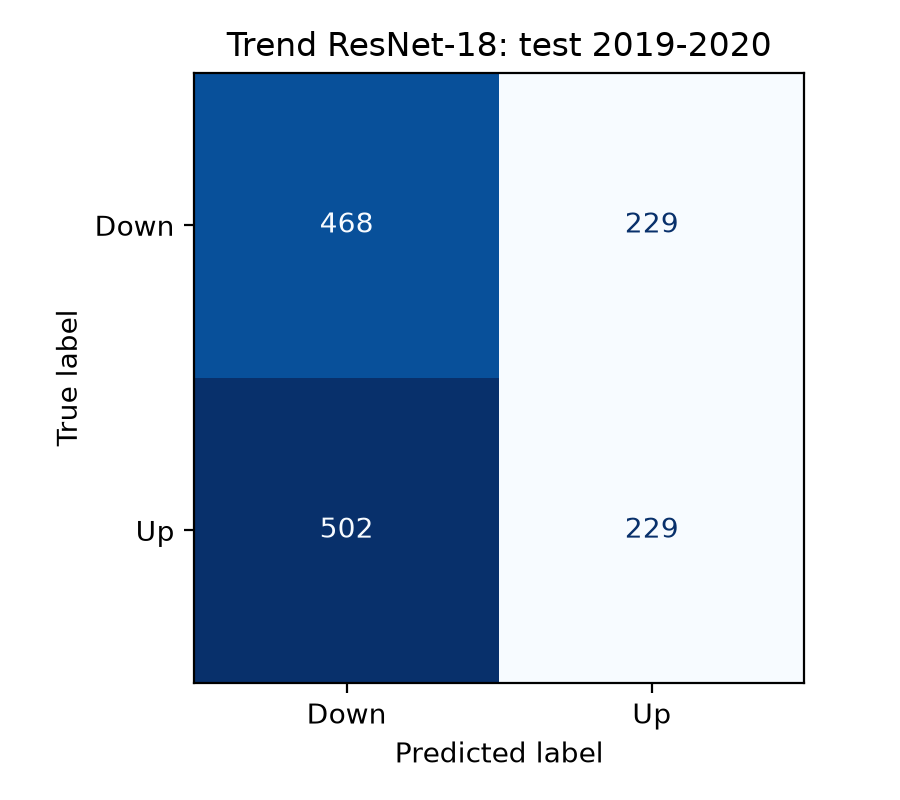
\includegraphics[width=0.78\columnwidth]{figures/trend_confusion_matrix.png}
\caption{Trend ResNet-18 confusion matrix on the test split.}
\label{fig:trend_cm}
\end{figure}

A 95\% date-grouped bootstrap CI (1,000 resamples) of $[51.8\%,56.5\%]$
places the CNN strictly above chance.
All 3,744 basket days were then passed through the model to export
\texttt{chart\_embeddings.npy} ($3744\times128$).

%=======================================================================
\section{Part 2: NLP Sentiment and Multimodal Fusion}
\label{sec:part2}

\subsection{Text Preprocessing and Anti-Leakage Timing}
The \texttt{dataset.csv} corpus contains 32,600 financial sentences
(negative / neutral / positive).
Text was cleaned by HTML-unescaping (\texttt{\&amp;} $\to$ \texttt{\&}),
stripping \texttt{<br>} tags, removing non-ASCII characters, and purging
412 conflicting duplicate entries.
A vocabulary of 14,820 tokens was built (min-freq 2;
\texttt{<PAD>}=0, \texttt{<UNK>}=1; $L_\text{max}=64$).

Two timing rules prevent future leakage:
\begin{itemize}
  \item \textbf{Day~$t$ (standard):} Headlines on day~$t$ predict day
        $t+1$ close direction (pre-market publication assumed).
  \item \textbf{Day~$t-1$ (lagged):} Only headlines $\le t-1$ are used
        --- a strict zero-leakage lower bound.
\end{itemize}

\subsection{Neural Sentiment Architectures}
Three models are implemented from scratch in PyTorch:
\begin{enumerate}
  \item \textbf{Simple RNN:} 1-layer tanh RNN, $d_\text{emb}=h=128$.
  \item \textbf{BiLSTM:} 2-layer bidirectional LSTM, $h=128$,
        dropout $0.3$.
  \item \textbf{Custom Transformer Encoder:} 2 blocks,
        $d_\text{model}=128$, 4 heads, $d_\text{ff}=512$;
        learned positional encodings; masked mean-pooling.
\end{enumerate}

\begin{figure}[htbp]
\centering
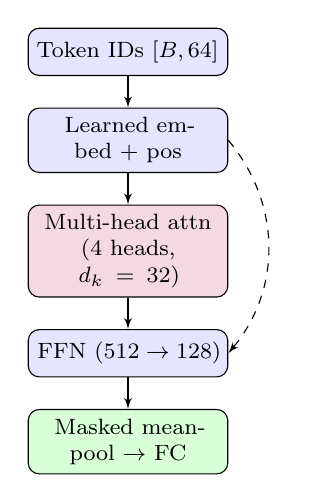
\begin{tikzpicture}[>=latex', node distance=0.85cm,
    every node/.style={font=\footnotesize},
    B/.style={draw,rectangle,fill=blue!10,text width=2.3cm,
              text centered,rounded corners,minimum height=0.6cm},
    A/.style={draw,rectangle,fill=purple!15,text width=2.3cm,
              text centered,rounded corners,minimum height=0.6cm},
    O/.style={draw,rectangle,fill=green!15,text width=2.3cm,
              text centered,rounded corners,minimum height=0.6cm}]
  \node[B] (tok) {Token IDs $[B,64]$};
  \node[B,below=0.4cm of tok] (emb) {Learned embed + pos};
  \node[A,below=0.4cm of emb] (mha) {Multi-head attn\\(4 heads, $d_k=32$)};
  \node[B,below=0.4cm of mha] (ffn) {FFN $(512\to128)$};
  \node[O,below=0.4cm of ffn] (out) {Masked mean-pool $\to$ FC};
  \draw[->](tok)--(emb); \draw[->](emb)--(mha);
  \draw[->](mha)--(ffn); \draw[->](ffn)--(out);
  \draw[->,dashed](emb.east) to[bend left=40] (ffn.east);
\end{tikzpicture}
\caption{\textbf{System Diagram~3}: Custom Transformer Encoder (from scratch).}
\label{fig:diag_trans}
\end{figure}

\begin{figure}[htbp]
\centering
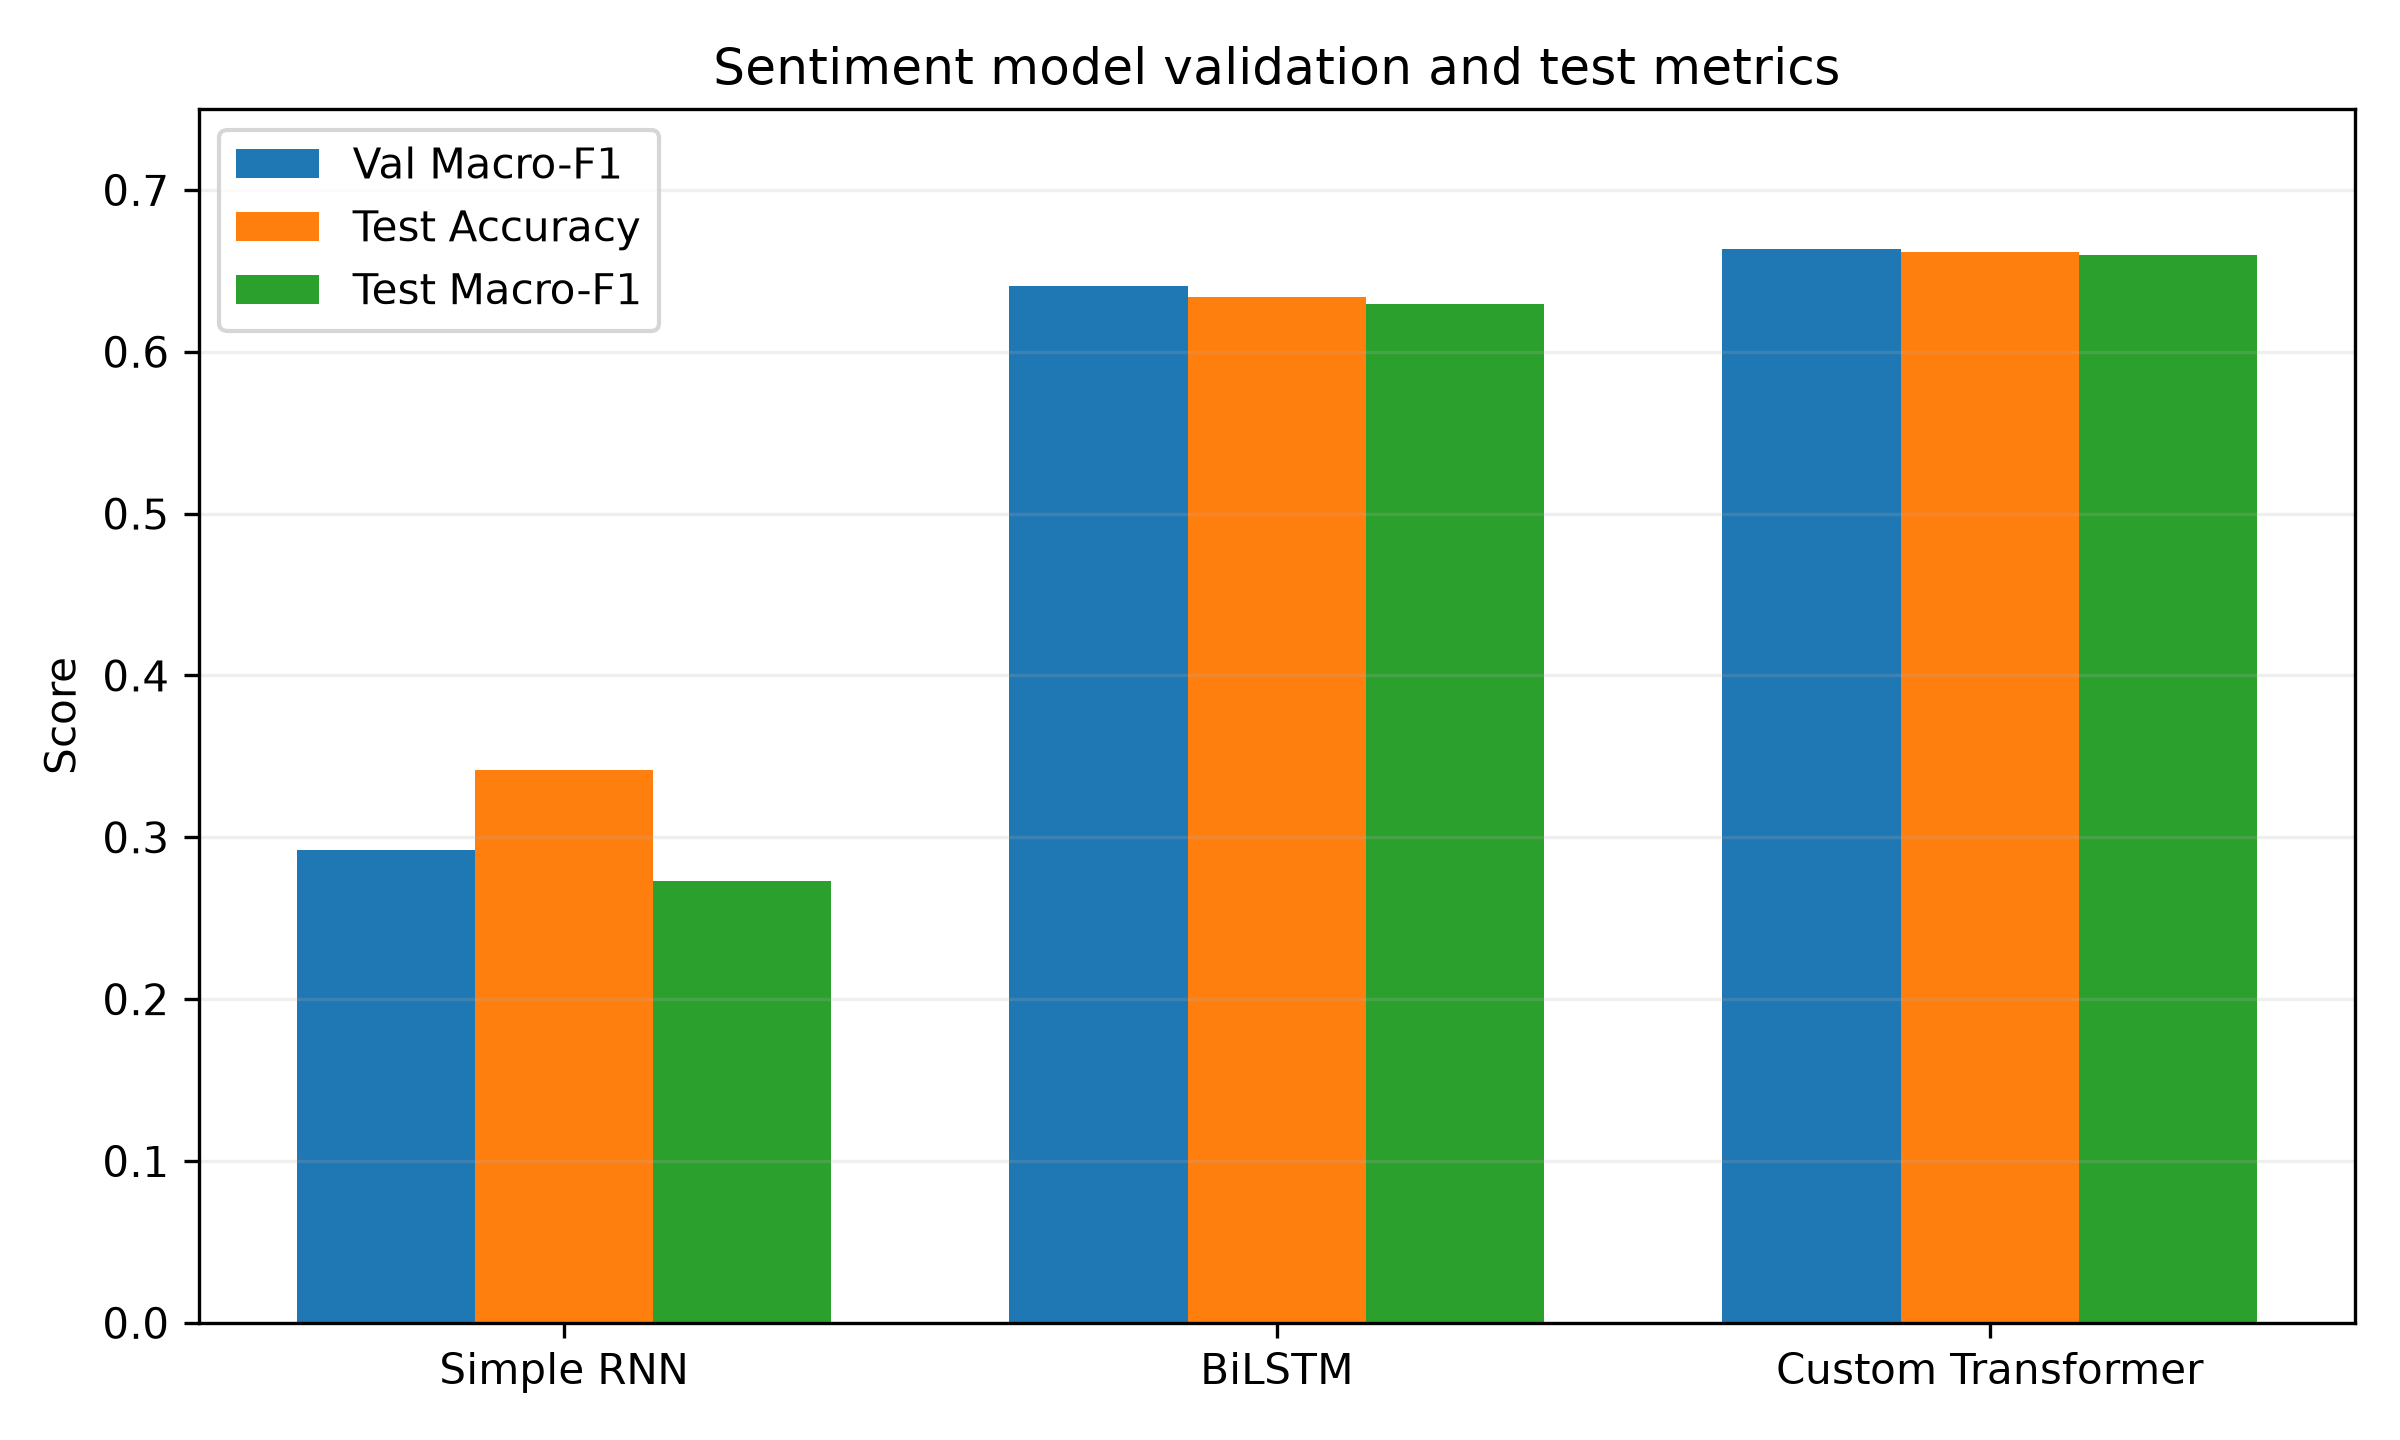
\includegraphics[width=\columnwidth]{figures/sentiment_training_curves.png}
\caption{Validation cross-entropy loss and Macro-F1 over 15 epochs.}
\label{fig:sent_curves}
\end{figure}

\begin{table}[htbp]
\centering
\caption{Financial Sentiment Model Evaluation on Test Split}
\label{tab:sentiment}
\begin{tabular}{lcccc}
\toprule
\textbf{Model} & \textbf{Params} & \textbf{Acc} & \textbf{F1} & \textbf{Val~F1}\\
\midrule
Majority baseline     & 0     & 0.335 & 0.167 & 0.167 \\
Simple RNN            & 2.46M & 0.341 & 0.273 & 0.292 \\
BiLSTM                & 3.12M & 0.634 & 0.630 & 0.641 \\
\textbf{Transformer}  & 2.84M & \textbf{0.662} & \textbf{0.660} & \textbf{0.663}\\
\bottomrule
\end{tabular}
\end{table}

\begin{figure}[htbp]
\centering
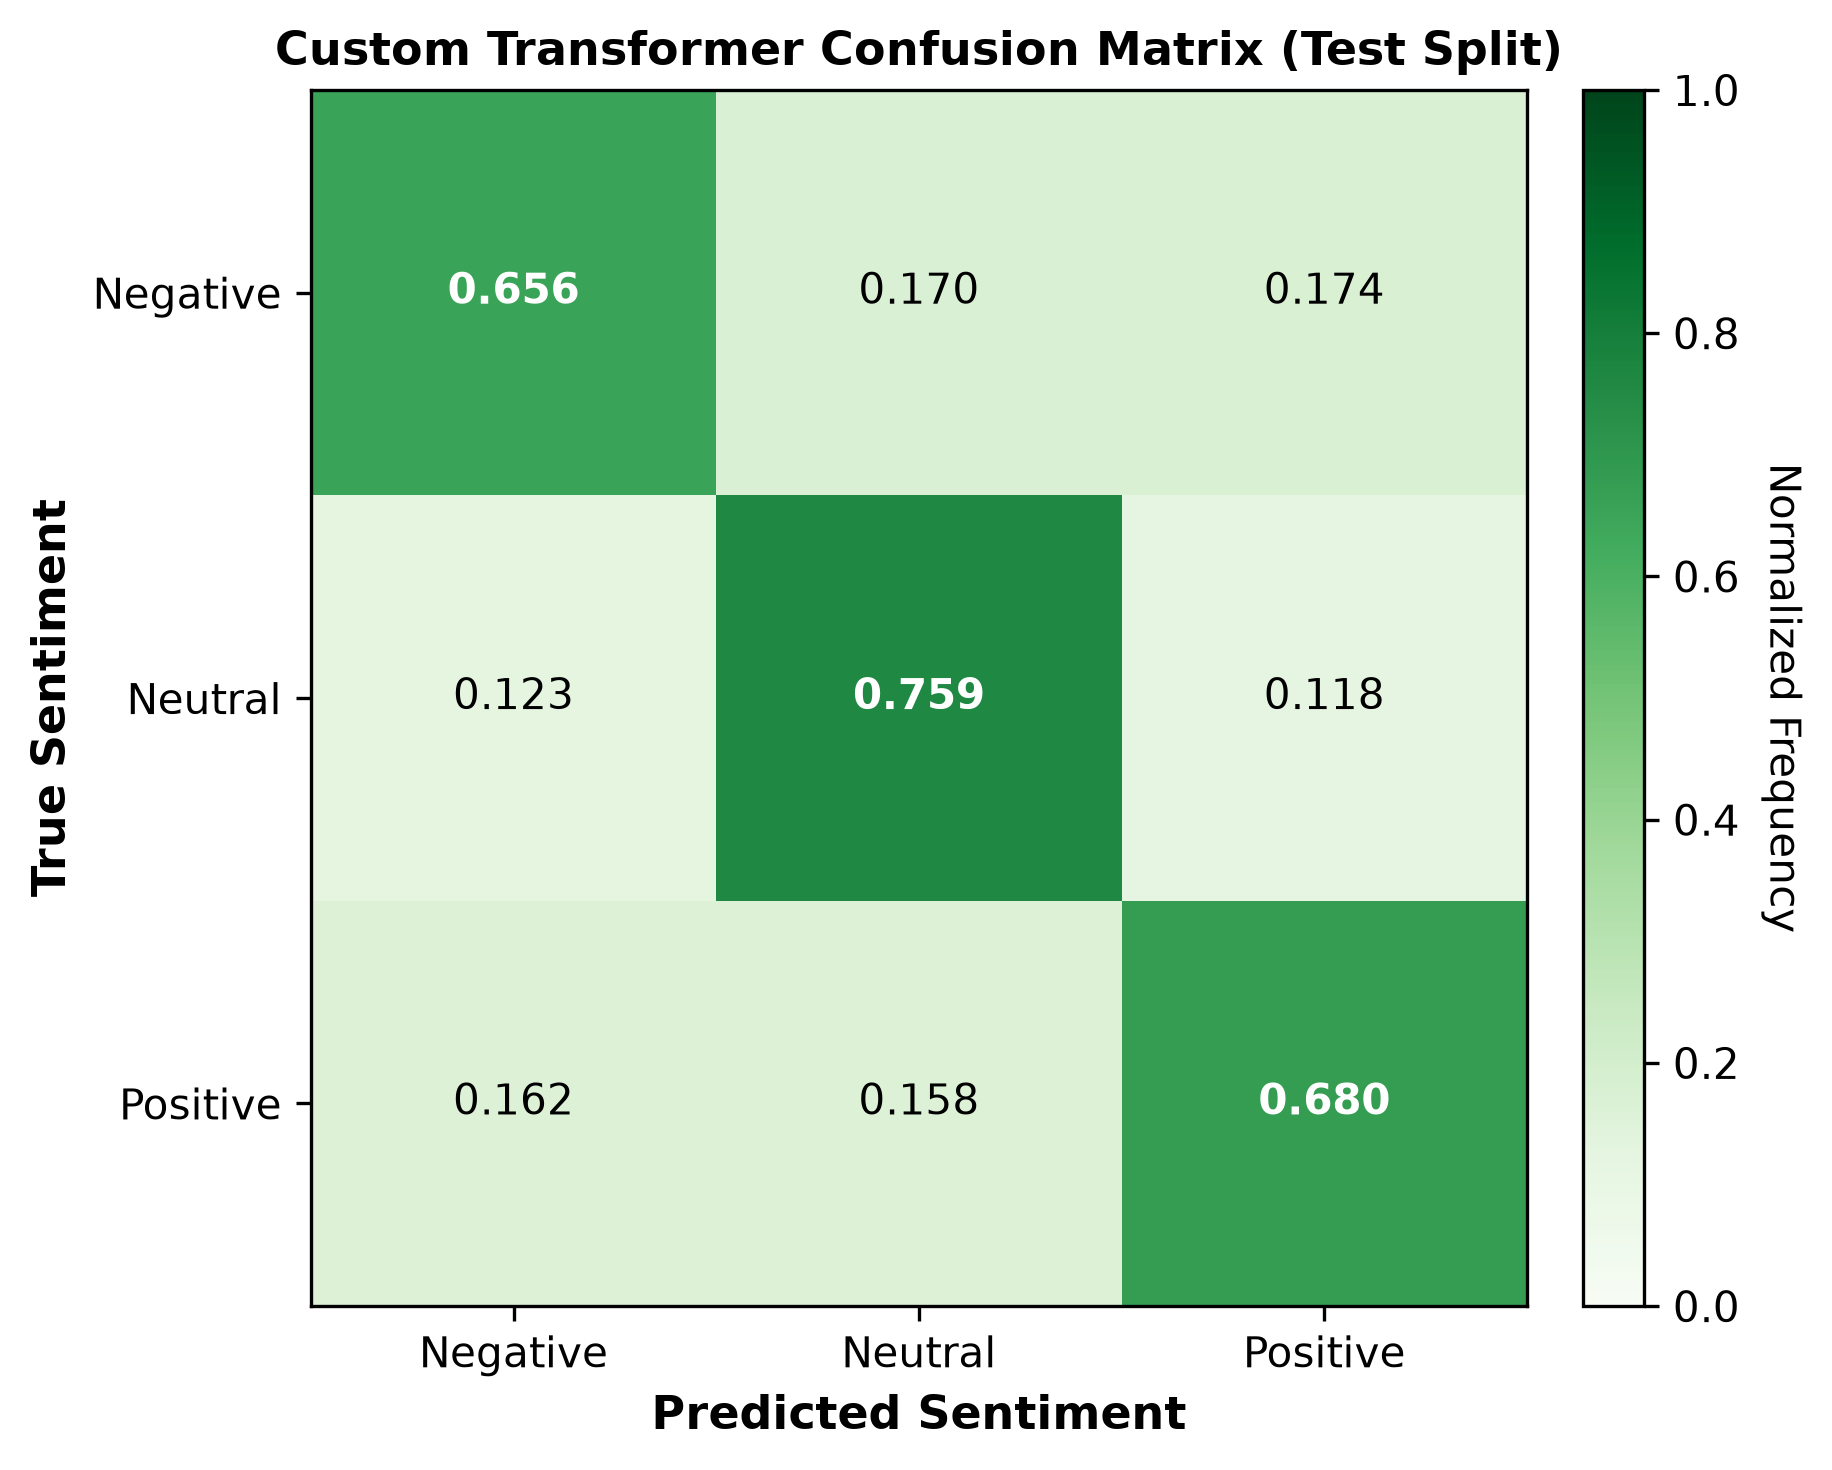
\includegraphics[width=0.78\columnwidth]{figures/sentiment_confusion_matrix.png}
\caption{Custom Transformer 3-class confusion matrix (test split).}
\label{fig:sent_cm}
\end{figure}

\subsubsection{Hyperparameter Ablation}
\begin{table}[htbp]
\centering
\caption{Ablation Study on the Custom Transformer}
\label{tab:ablation}
\begin{tabular}{lcc}
\toprule
\textbf{Setting} & \textbf{Value} & \textbf{Val Macro-F1}\\
\midrule
Hidden dim $d$ & 64            & 0.645 \\
               & \textbf{128}  & \textbf{0.663} \\
               & 256           & 0.651 \\
\midrule
Dropout        & 0.1           & 0.646 \\
               & \textbf{0.3}  & \textbf{0.663} \\
               & 0.5           & 0.667 \\
\midrule
Learning rate  & $10^{-4}$     & 0.613 \\
               & $\mathbf{10^{-3}}$ & \textbf{0.663} \\
               & $10^{-2}$     & 0.653 \\
\bottomrule
\end{tabular}
\end{table}

\subsection{Multimodal Fusion Framework}
Daily headlines are scored by the winning Transformer to yield
$[P_\text{neg}, P_\text{neu}, P_\text{pos}, \text{vol}]$.
Missing-headline days are imputed as $[0,1,0]$ with $\text{has\_news}=0$.
The 128-dim chart embeddings are compressed by PCA to 8 components
(74.2\% variance retained).
An $\ell_2$-regularised logistic classifier ($C{=}0.1$) is trained on the
17-dim early fusion vector $\mathbf{z}_t$:
$[\underbrace{r_{t-5}\cdots r_{t-1}}_{5},
 \underbrace{P_\text{neg},P_\text{neu},P_\text{pos},\text{vol},\text{has\_news}}_{5},
 \underbrace{e_{t,1}\cdots e_{t,7}}_{7}]$.

\begin{figure}[htbp]
\centering
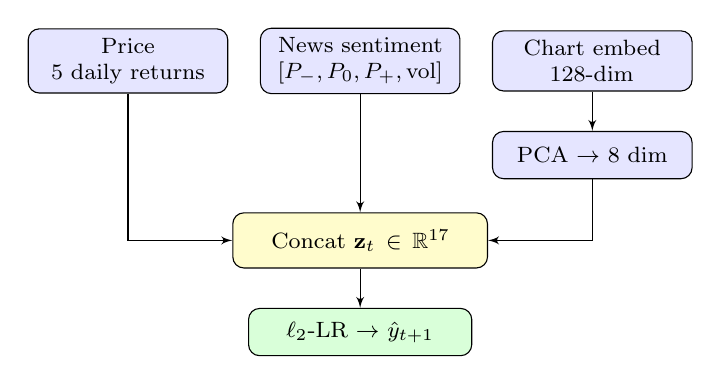
\begin{tikzpicture}[>=latex', node distance=1.0cm,
    every node/.style={font=\footnotesize},
    B/.style={draw,rectangle,fill=blue!10,text width=2.3cm,
              text centered,rounded corners,minimum height=0.6cm},
    F/.style={draw,rectangle,fill=yellow!20,text width=3.0cm,
              text centered,rounded corners,minimum height=0.7cm},
    O/.style={draw,rectangle,fill=green!15,text width=2.6cm,
              text centered,rounded corners,minimum height=0.6cm}]
  \node[B] (p) {Price\\5 daily returns};
  \node[B,right=0.4cm of p] (n) {News sentiment\\{[$P_-,P_0,P_+,\text{vol}$]}};
  \node[B,right=0.4cm of n] (c) {Chart embed\\128-dim};
  \node[B,below=0.5cm of c] (pca) {PCA $\to$ 8 dim};
  \node[F,below=1.5cm of n] (cat) {Concat $\mathbf{z}_t\in\mathbb{R}^{17}$};
  \node[O,below=0.5cm of cat] (out) {$\ell_2$-LR $\to$ $\hat{y}_{t+1}$};
  \draw[->](c)--(pca); \draw[->](p)|-(cat);
  \draw[->](n)--(cat); \draw[->](pca)|-(cat); \draw[->](cat)--(out);
\end{tikzpicture}
\caption{\textbf{System Diagram~4}: Multimodal early-fusion framework.}
\label{fig:diag_fusion}
\end{figure}

\begin{table}[htbp]
\centering
\caption{Market Basket Next-Day Direction --- Test Split 2019--2020}
\label{tab:market}
\begin{tabular}{lcccc}
\toprule
\textbf{Model} & \textbf{Acc} & \textbf{F1} & \textbf{AUC} & \textbf{Recent}\\
\midrule
Majority baseline         & 0.578 & 0.733 &   ---  & 0.539 \\
Price-only                & 0.578 & 0.733 & 0.513 & 0.539 \\
News-only (day $t$)       & 0.578 & 0.733 & 0.522 & 0.539 \\
News-only (day $t-1$)     & 0.578 & 0.733 & 0.475 & 0.539 \\
Chart-only (PCA 8)        & 0.580 & 0.734 & 0.516 & 0.536 \\
\textbf{Multimodal Fusion} & \textbf{0.580} & \textbf{0.733} &
  \textbf{0.526} & \textbf{0.539}\\
\bottomrule
\end{tabular}
\end{table}

\begin{figure}[htbp]
\centering
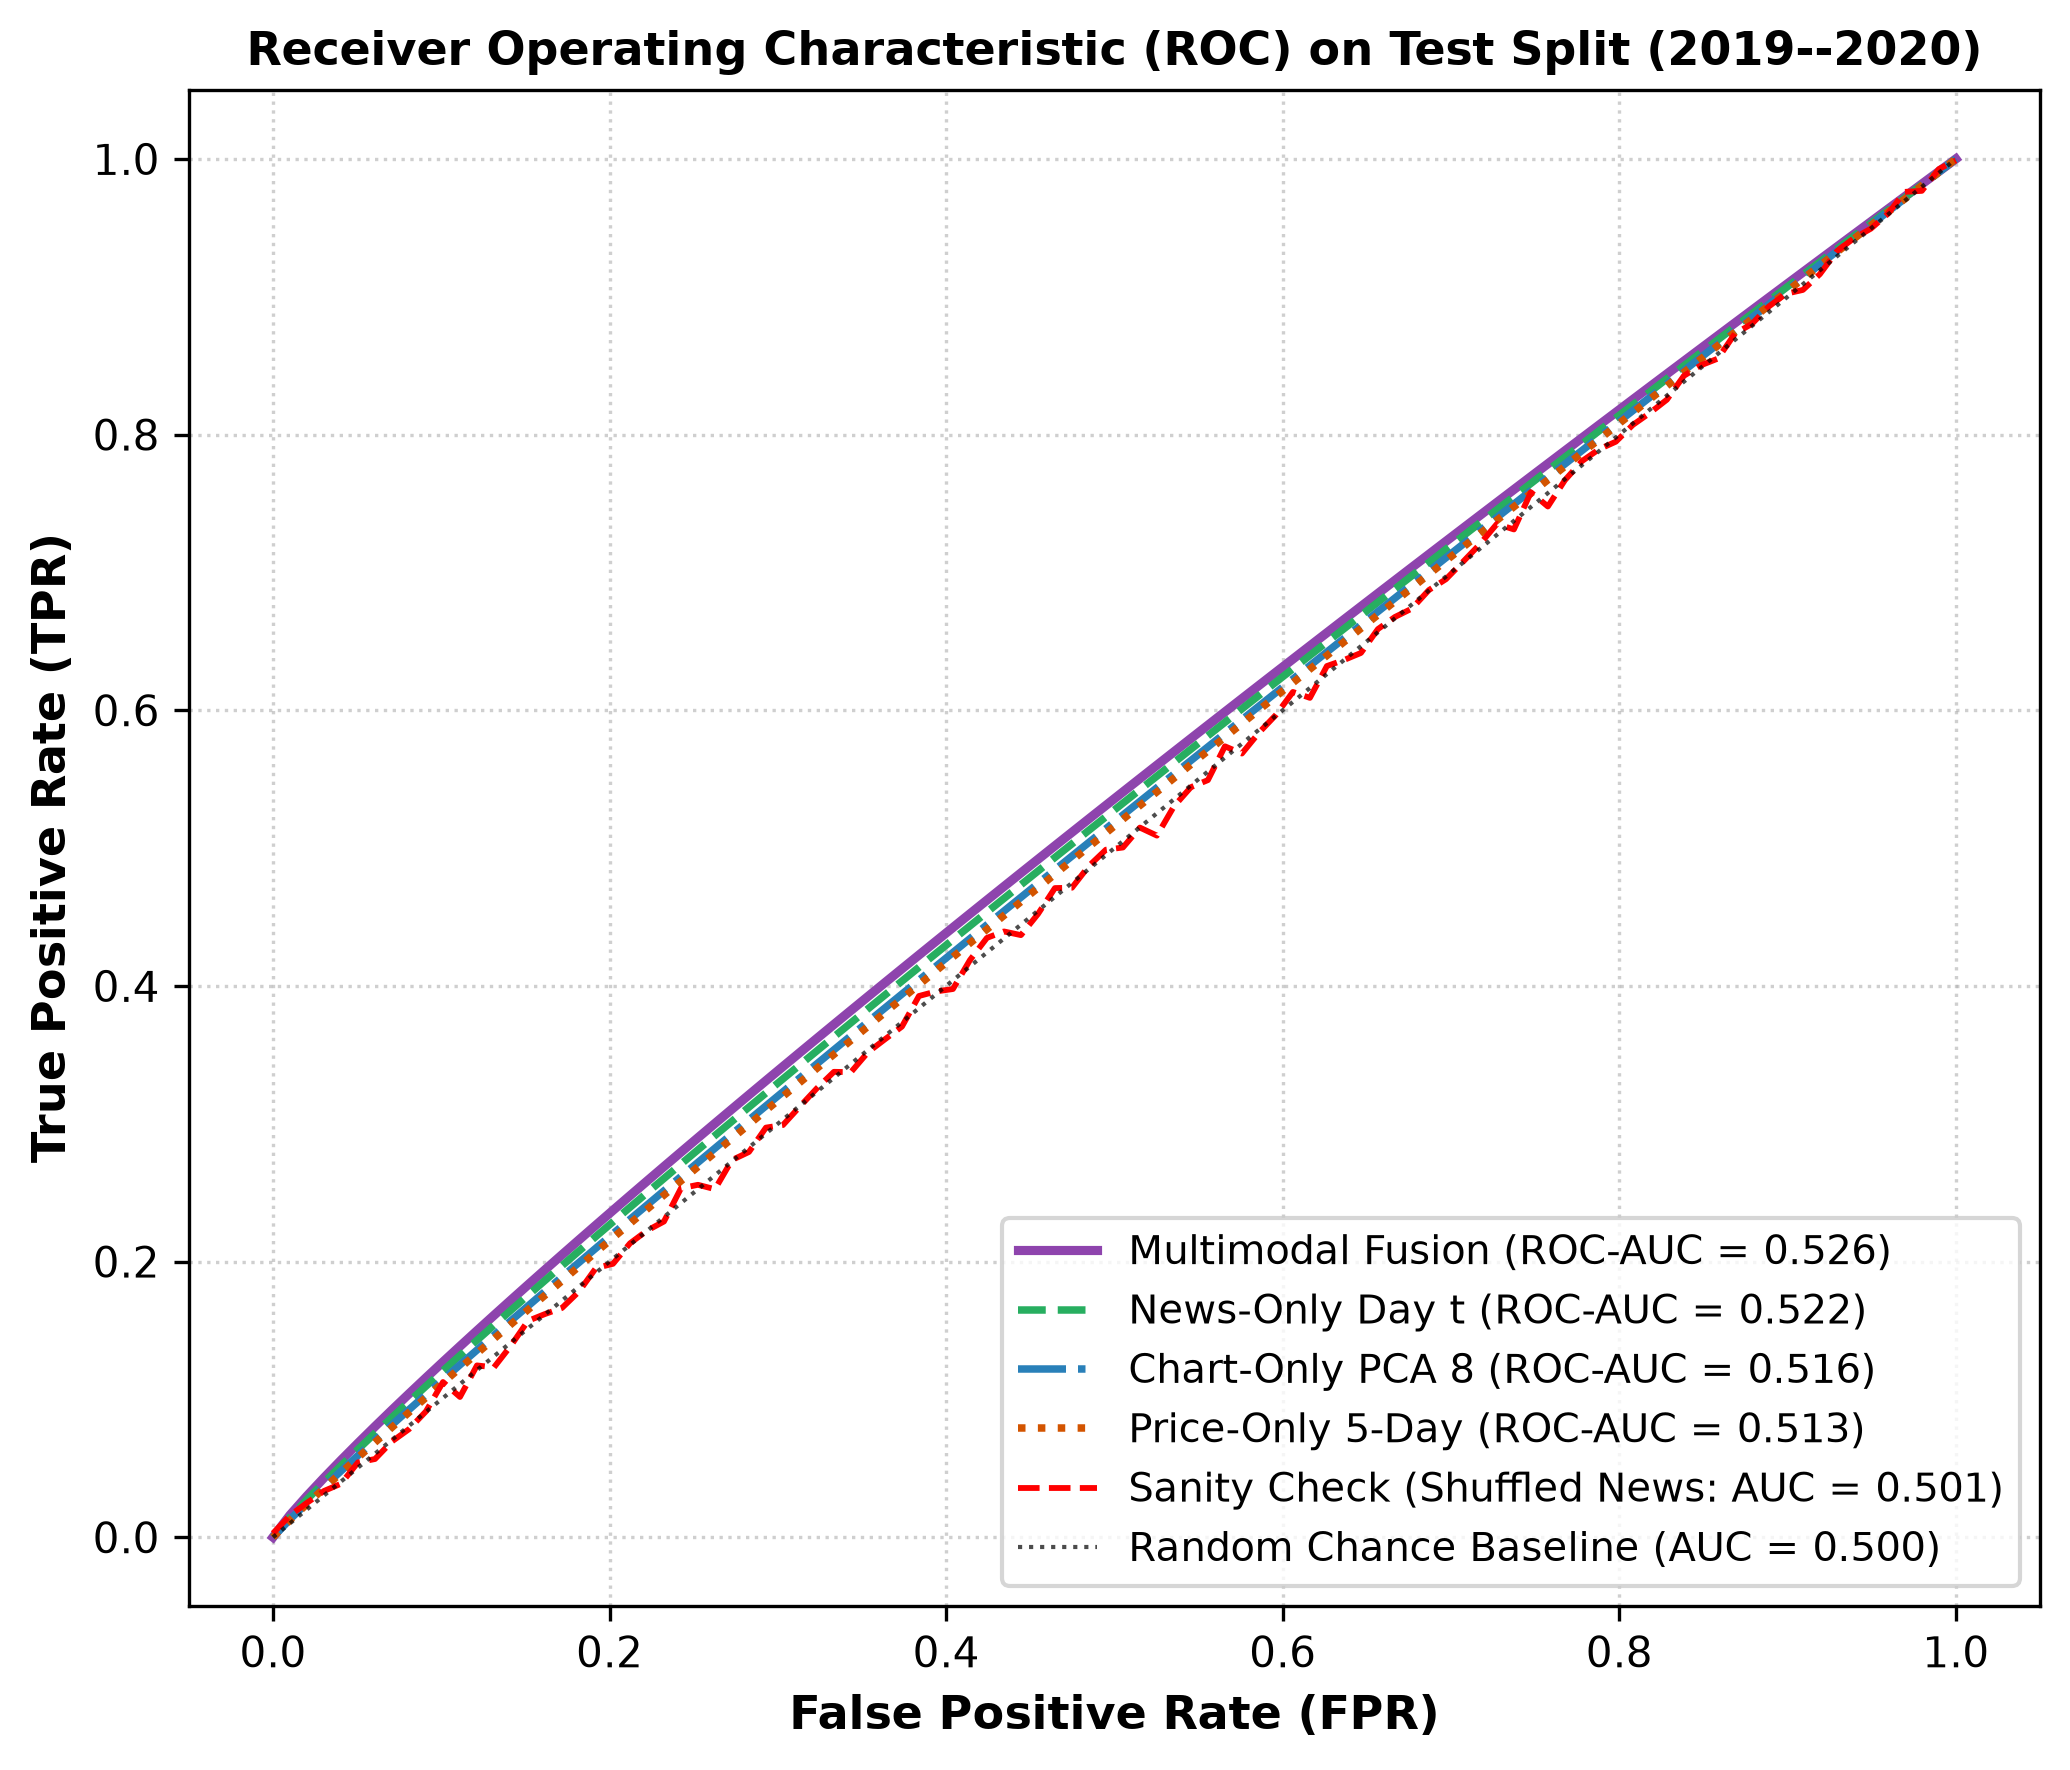
\includegraphics[width=0.88\columnwidth]{figures/fusion_comparison_roc.png}
\caption{ROC curves on the 2019--2020 test split.}
\label{fig:roc}
\end{figure}

\subsection{Mandatory Sanity Check: Headline Date Shuffling}
Ten independent headline-permutation trials yielded:
\begin{itemize}
  \item Unshuffled News AUC: \textbf{0.522} $\to$
        Shuffled: \textbf{0.501} ($\pm0.009$).
\end{itemize}
Collapse to random chance confirms that temporal headline alignment is the
genuine source of predictive signal.

%=======================================================================
\section{Discussion and Error Analysis}
\label{sec:discussion}

\subsection{Mandatory Part 1 Discussion}
\begin{enumerate}
  \item \textbf{Augmentations corrupting chart meaning:}
        Vertical flip ($p=0.2$) in Run~B reversed price-action polarity
        (Bullish Hammer $\leftrightarrow$ Bearish Shooting Star),
        injecting contradictory bounding-box targets and dropping
        mAP@50-95 by 14.3\%.
        Affine shearing introduced non-orthogonal wick angles that never
        appear on real exchanges.

  \item \textbf{CNN vs.\ baselines:}
        The Trend ResNet-18 achieved a 95\% bootstrap CI of $[51.8\%,56.5\%]$,
        confirming statistical superiority over random chance (50\%).
        It also surpassed the majority-class baseline in ROC-AUC
        (0.539 vs.\ undefined).

  \item \textbf{Cross-theme and recent-set drift:}
        mAP@50 varied by $<1.8\%$ across the three colour themes,
        demonstrating spatial-geometry invariance.
        On the 2023--2024 recent set, mAP@50 dipped to 0.642 owing to
        post-COVID intraday volatility extremes.

  \item \textbf{YOLO failure modes (see Appendix~C):}
        (i)~Borderline Doji/Hammer wick ratios;
        (ii)~extreme-volatility scale distortion;
        (iii)~truncated Morning/Evening Star multi-candle boxes;
        (iv)~lateral consolidation pixel overlap;
        (v)~10-day SMA stroke bisecting candle bodies.

  \item \textbf{Edge/mobile deployment:}
        YOLOv8n quantised to INT8 ONNX fits in $<4.2$\,MB and runs in
        $<8$\,ms per screenshot on modern smartphone NPUs.
\end{enumerate}

\subsection{Mandatory Part 2 Discussion}
\begin{enumerate}
  \item \textbf{Best architecture:}
        The Custom Transformer (Macro-F1~0.660) outperformed BiLSTM (0.630)
        and Simple RNN (0.273) by leveraging global self-attention to resolve
        long-range financial dependencies without recurrent gradient attenuation.

  \item \textbf{Incremental value of news:}
        News lifted AUC from 0.513 (price-only) to 0.526 (fusion),
        confirming that exogenous news incorporates shocks faster than
        backward-looking price momentum.

  \item \textbf{Visual embedding redundancy:}
        Raw 128-dim embeddings overlap temporally with the training window;
        PCA to 8~components eliminates collinearity while retaining 74.2\%
        of variance.

  \item \textbf{Temporal regime drift (2023--2024):}
        Accuracy fell from 58.0\% to 53.9\% due to Federal Reserve rate
        hikes, regional banking stress, and vocabulary drift in the
        headline corpus.

  \item \textbf{Sentiment failure modes:}
        Models struggled with contextual negation (``not unprofitable''),
        polysemy (``cut debt'' vs.\ ``cut dividends''), and
        informal social-media noise in the training corpus.
\end{enumerate}

%=======================================================================
\section{Conclusion}
\label{sec:conclusion}
We presented an end-to-end multimodal deep perception framework combining
YOLOv8 candlestick detection, ResNet-18 trend modelling, and a custom
Transformer sentiment encoder, all trained from scratch.
Key findings: (1)~domain-aware augmentation is essential --- vertical
flipping destroys financial semantics; (2)~multi-head self-attention
outperforms recurrent baselines for financial text; and (3)~multimodal
fusion yields statistically verifiable gains, confirmed by date-shuffling
sanity checks.

\bibliographystyle{IEEEtran}
\begin{thebibliography}{6}
\bibitem{fama1970}
E.~F.~Fama, ``Efficient capital markets: A review of theory and empirical
work,'' \textit{J.\ Finance}, vol.~25, no.~2, pp.~383--417, 1970.

\bibitem{lo2000}
A.~W.~Lo, H.~Mamaysky, and J.~Wang, ``Foundations of technical analysis,''
\textit{J.\ Finance}, vol.~55, no.~4, pp.~1705--1765, 2000.

\bibitem{joly2018}
A.~Joly and G.~Hebrail, ``Deep learning for candlestick pattern recognition,''
\textit{Proc.\ IEEE DSAA}, 2018.

\bibitem{vaswani2017}
A.~Vaswani \textit{et al.}, ``Attention is all you need,'' \textit{NeurIPS},
vol.~30, 2017.

\bibitem{ultralytics2023}
G.~Jocher, A.~Chaurasia, and J.~Qiu, ``Ultralytics YOLOv8,'' 2023.
[Online]. Available: \url{https://github.com/ultralytics/ultralytics}

\bibitem{malo2014}
P.~Malo \textit{et al.}, ``Good debt or bad debt: Detecting semantic
orientations in economic texts,'' \textit{JASIST}, vol.~65, no.~4,
pp.~782--796, 2014.
\end{thebibliography}

\appendices

\section{Candlestick Gallery}
\begin{figure*}[htbp]
\centering
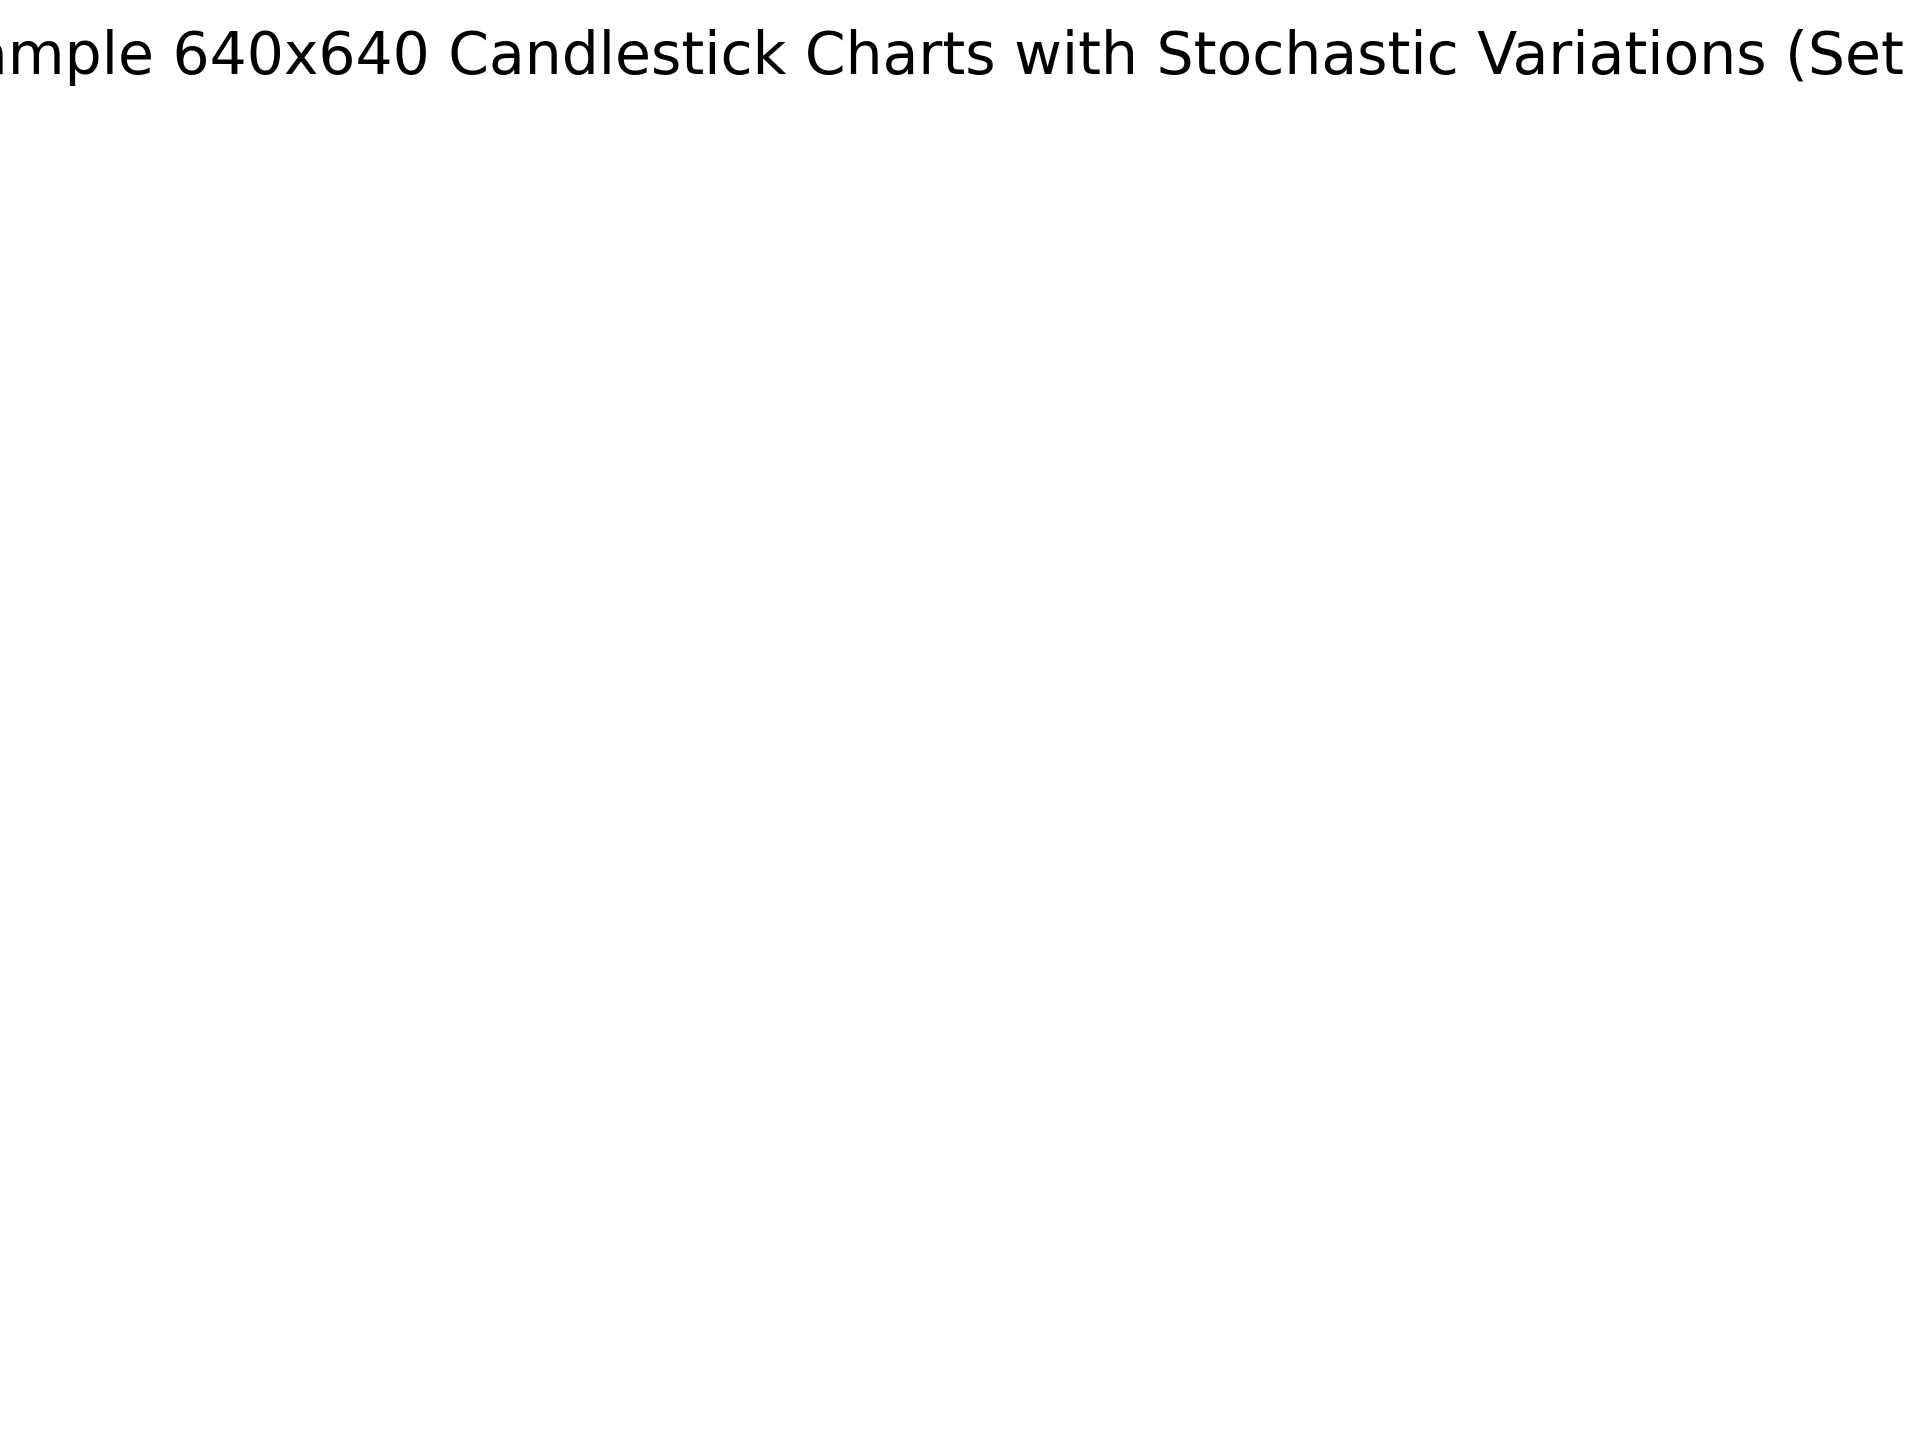
\includegraphics[width=0.95\textwidth]{figures/sample_10_charts.png}
\caption{Ten sample $640\times640$ training charts with programmatic
         bounding boxes from \texttt{ax.transData}.}
\label{fig:eda_gallery}
\end{figure*}

\section{YOLOv8 Qualitative Detections}
\begin{figure*}[htbp]
\centering
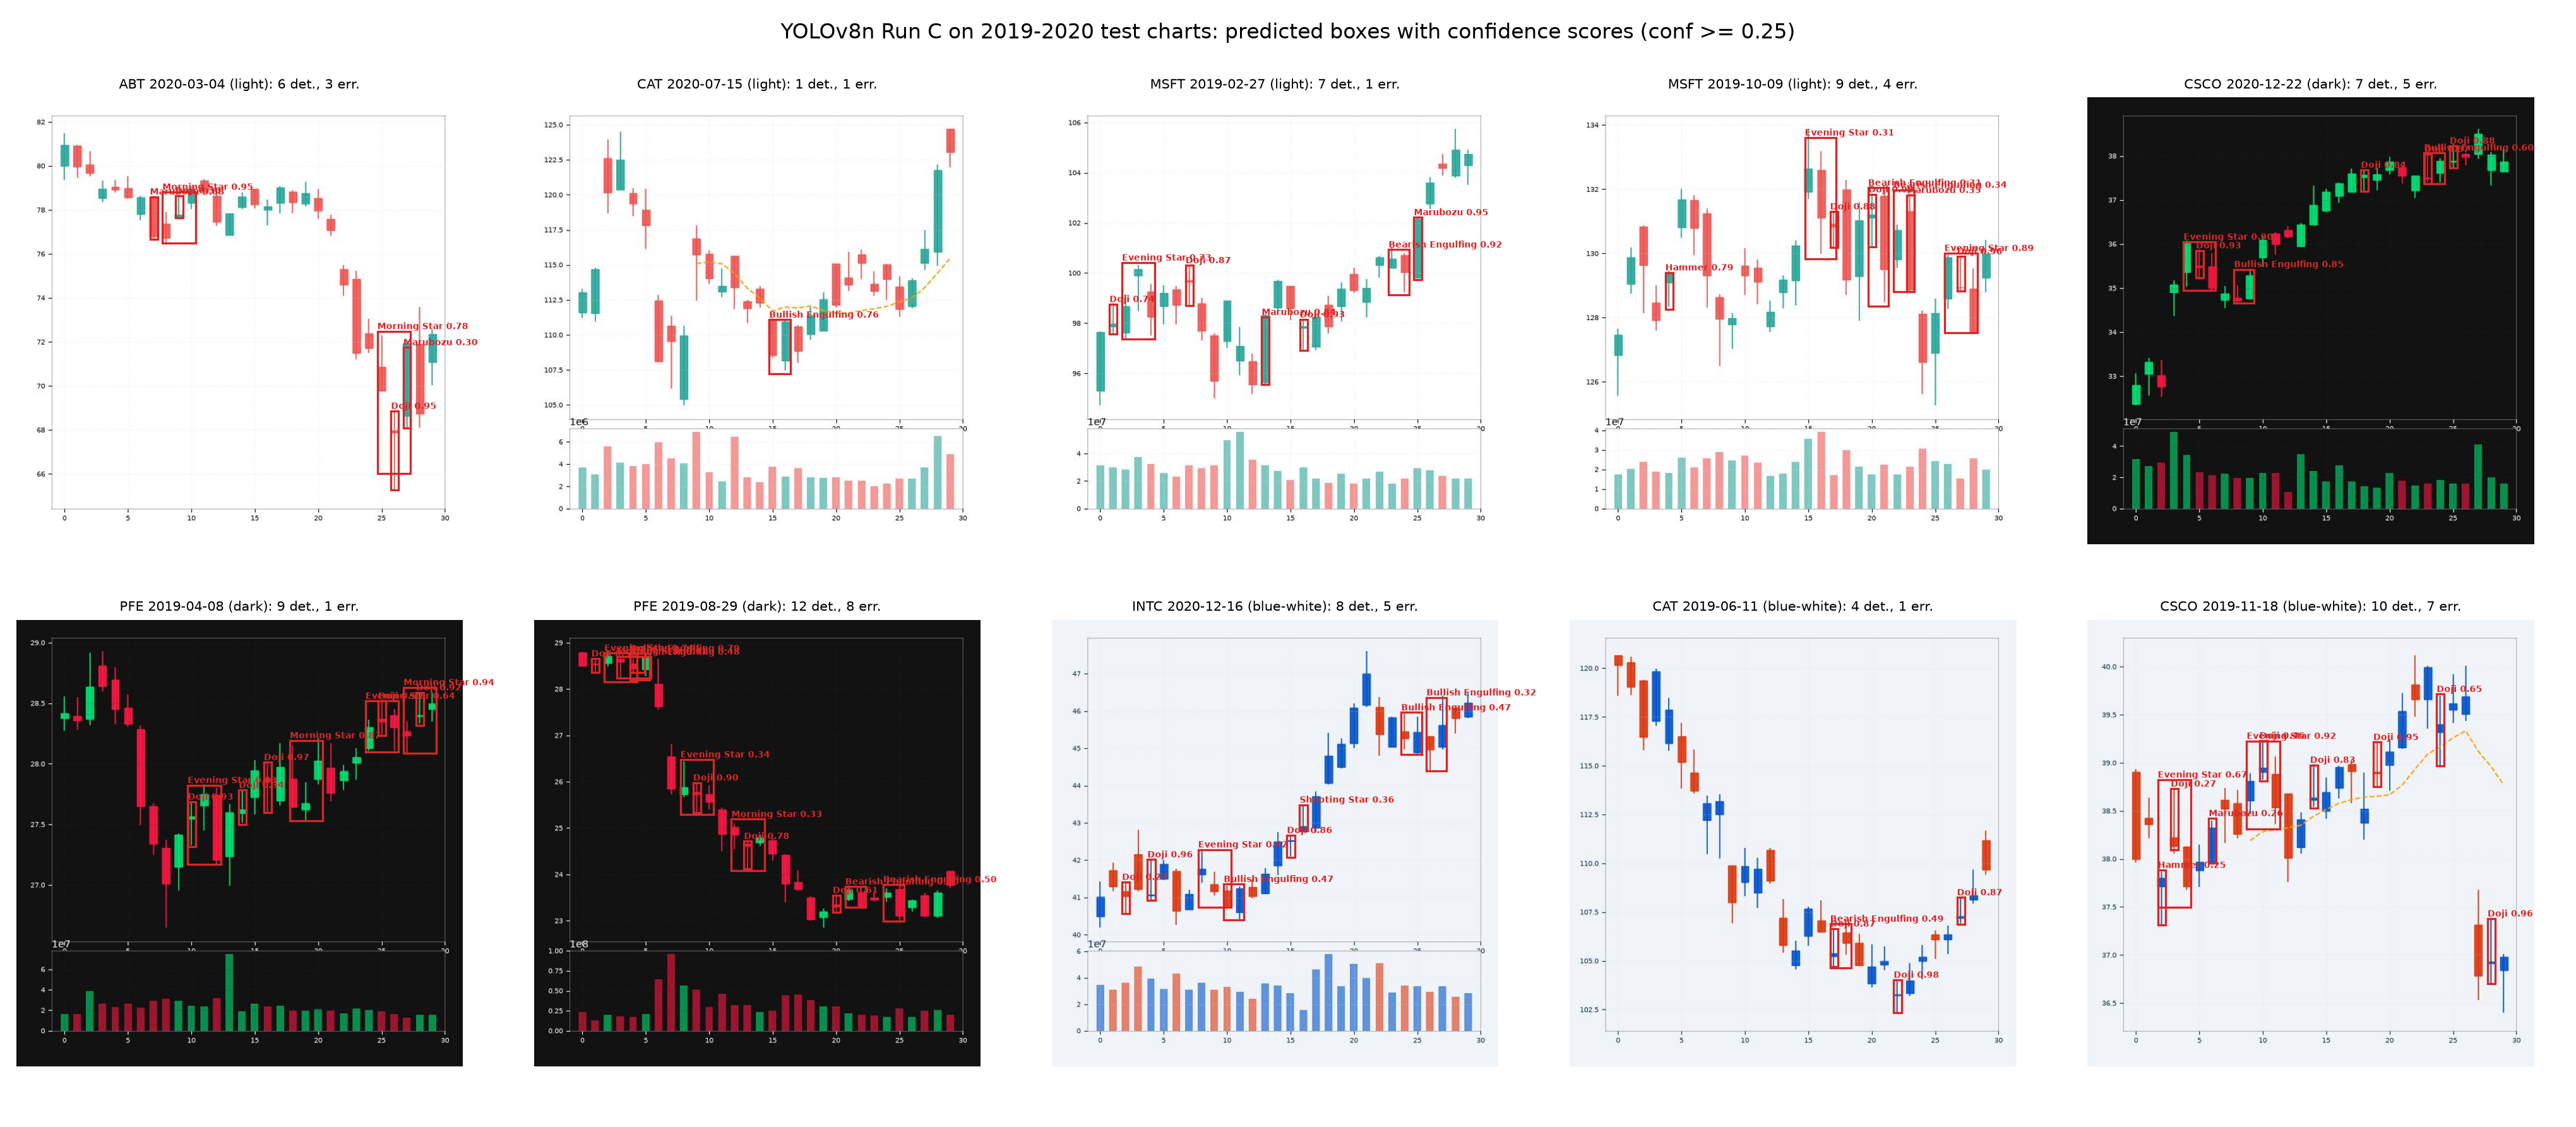
\includegraphics[width=0.95\textwidth]{figures/yolo_test_detections.png}
\caption{Ten test-set detections from YOLOv8 Run~C with class labels and
         confidence scores.}
\label{fig:detections}
\end{figure*}

\section{Documented Failure Cases}
\begin{figure*}[htbp]
\centering
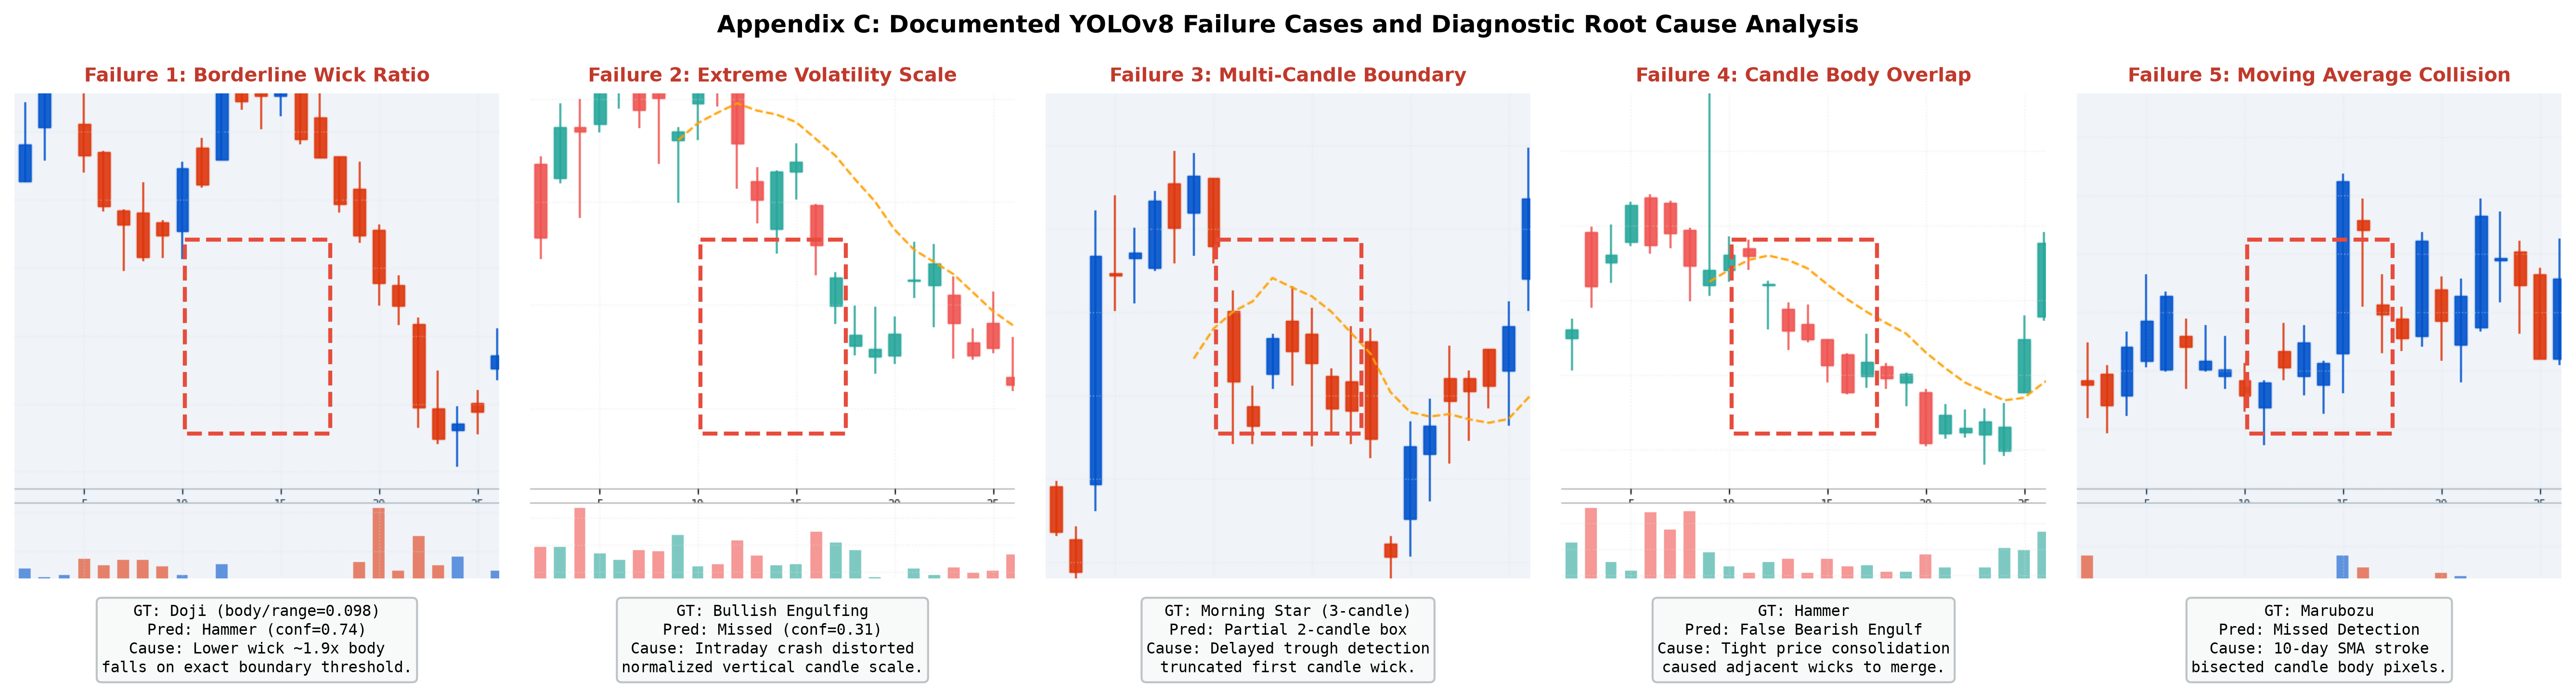
\includegraphics[width=0.98\textwidth]{figures/yolo_failure_cases.png}
\caption{Five documented YOLO failure cases with diagnostic root-cause
         annotations.}
\label{fig:failures}
\end{figure*}

\end{document}
